% main.tex
% Fichero principal de transparencias (incluye a todos los dem�s).

% Compilar a .pdf con LaTeX (pdflatex)
% Es necesario instalar Beamer (paquete latex-beamer en Debian)
%

% Gr�ficos:
% Los gr�ficos pueden suministrarse en PNG, JPG, TIF, PDF, MPS
% Los EPS deben convertirse a PDF (usar epstopdf)
%
\documentclass{beamer}
\usetheme{Warsaw}
\beamertemplatenavigationsymbolsempty
\setbeamertemplate{headline}{}
%\useoutertheme{infolines}
%\usebackgroundtemplate{
\includegraphics[width=\paperwidth]{format/libresoft-bg-soft.png}}
\usepackage[spanish]{babel}
\usepackage[latin1]{inputenc}
\usepackage{graphics}
\usepackage{amssymb} % Simbolos matematicos

\newcommand{\asignatura}{Servicios y Aplicaciones Telem�ticas}
\newcommand{\grado}{Grado en Ingenier�a Tecnolog�as de Telecomunicaci�n (URJC)}
\newcommand{\curso}{2014-15}
\newcommand{\horario}{M (11:00-13:00) y J (11:00-13:00)}

%\definecolor{libresoftgreen}{RGB}{162,190,43}
%\definecolor{libresoftblue}{RGB}{0,98,143}

%\setbeamercolor{titlelike}{bg=libresoftgreen}

%% Metadatos del PDF.
\hypersetup{
  pdftitle={\asignatura~\curso},
  pdfauthor={Jes�s M. Gonz�lez Barahona, Gregorio Robles},
  pdfcreator={GSyC, Universidad Rey Juan Carlos},
  pdfproducer=PDFLaTeX,
  pdfsubject={\asignatura~\curso},
}
%%

%%%%%%%%%%%%%%%%%%%%%%%%%%%%%%%%%%%%%%%%%%%%%%%%%%%%%%%%%%%%%%%%
%%%%%%%%%%%%%%%%%%%%%%%%%%%%%%%%%%%%%%%%%%%%%%%%%%%%%%%%%%%%%%%%
% include-only                                                 %
%%%%%%%%%%%%%%%%%%%%%%%%%%%%%%%%%%%%%%%%%%%%%%%%%%%%%%%%%%%%%%%%
%%%%%%%%%%%%%%%%%%%%%%%%%%%%%%%%%%%%%%%%%%%%%%%%%%%%%%%%%%%%%%%%
\includeonly{presentacion-sat-saro}
%\includeonly{presentacion, html}
%\includeonly{html}
%\includeonly{html5}

%% Pr�cticas
%\includeonly{html}
%\includeonly{css}
%\includeonly{css3}
%\includeonly{html5}
%\includeonly{gapi}

\AtBeginSection[]
{
\begin{frame}<beamer>
\begin{center}
{\Huge \insertsection}
\end{center}
\end{frame}
}

\begin{document}

\title[\asignatura~\curso]{\asignatura~(\curso)}
\subtitle{\grado}
\author[GSyC]{Jes�s M. Gonz�lez Barahona, Gregorio Robles Mart�nez}
\institute[http://cursosweb.github.io/]{\url{http://cursosweb.github.io} \\
GSyC, Universidad Rey Juan Carlos}

%\date{Enero 2015}

\frame{
\maketitle
}


% Si el titulo o el autor se quieren acortar para los pies de p�gina
% se pueden redefinir aqu�:
%\title{Titulo corto}
%\author{Autores abreviado}


%% LICENCIA DE REDISTRIBUCION DE LAS TRANSPAS
\frame{
~
\vspace{3cm}

\begin{flushright}
\copyright 2002-2015 Jes�s M. Gonz�lez Barahona, Gregorio Robles. \\

Algunos derechos reservados. Este art�culo se distribuye bajo
la licencia ``Reconocimiento-CompartirIgual 3.0 Espa�a'' de Creative Commons,
disponible en \\
{\small \url{http://creativecommons.org/licenses/by-sa/3.0/es/deed.es}}

Este documento (o uno muy similar) est� disponible en \\
\url{http://cursosweb.github.io}
\end{flushright}
}
%%

%%%%%%%%%%%%%%%%%%%%%%%%%%%%%%%%%%%%%%%%%%%%%%%%%%%%%%%%%%%%%%%%
%%%%%%%%%%%%%%%%%%%%%%%%%%%%%%%%%%%%%%%%%%%%%%%%%%%%%%%%%%%%%%%%
% lista de temas                                               %
%%%%%%%%%%%%%%%%%%%%%%%%%%%%%%%%%%%%%%%%%%%%%%%%%%%%%%%%%%%%%%%%
%%%%%%%%%%%%%%%%%%%%%%%%%%%%%%%%%%%%%%%%%%%%%%%%%%%%%%%%%%%%%%%%


\section{Presentaci�n de la asignatura}

%%---------------------------------------------------------------

\begin{frame}
\frametitle{Datos, datos, datos}

\begin{itemize}
\item Profesores:
  \begin{itemize}
  \item Jes�s M. Gonz�lez Barahona (jgb @ gsyc.urjc.es)
  \item Gregorio Robles (grex @ gsyc.urjc.es)
  \end{itemize}
\item Grupo de Sistemas y Comunicaciones (GSyC)
\item Despachos: 101 y 110 Departamental III
\item Horario: \horario
\item Tutor�a: Horario por definir (en los Laboratorios)
\item Laboratorio 209 Laboratorios III
\end{itemize}

\begin{flushright}
  Campus virtual: {\small \url{http://aulavirtual.urjc.es}} \\
  Cursos web: {\small \url{http://cursosweb.github.io}} \\
  GitLab de la ETSIT: {\small \url{http://gitlab.etsit.urjc.es}} \\
\end{flushright}

\end{frame}


%-----------------------    ---------------------------------
\usebackgroundtemplate{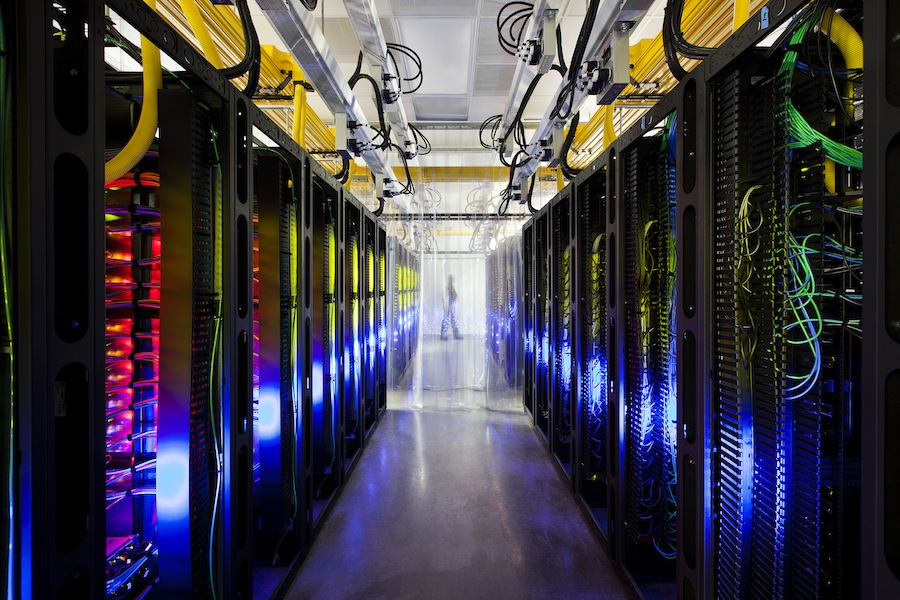
\includegraphics[width=12.8cm]{figs/internet.jpg}}
% http://cdn6.yorokobu.es/wp-content/uploads/Council-Bluffs-Network-Room.jpg

\begin{frame}
\frametitle{�De qu� va todo esto?}

\vspace{3.5cm}

\begin{center}
\color{white}
\Huge {\bf Entendiendo c�mo funciona la web}
\end{center}

\end{frame}
\usebackgroundtemplate{}


%%---------------------------------------------------------------

\begin{frame}
\frametitle{En concreto...}

{\Large
\begin{itemize}
\item C�mo se construyen los sistemas reales \\
  que se usan en Internet
  \item Qu� tecnolog�as se est�n usando
  \item Qu� esquemas de seguridad hay
  \item C�mo encajan las piezas
  \item En la medida de lo posible, ``manos en la masa''
\end{itemize}
}

\end{frame}


%%---------------------------------------------------------------

\begin{frame}
\frametitle{Ejemplos}

{\Large
\begin{itemize}
  \item �Qu� es una aplicaci�n web?
  \item �Qu� es una sesi�n?
  \item �C�mo construir un servicio REST?
  \item Acaba con la magia de los servicios web
  \item �C�mo se hace un servicio basado en contenidos?
\end{itemize}
}
\end{frame}

%-----------------------    ---------------------------------
\usebackgroundtemplate{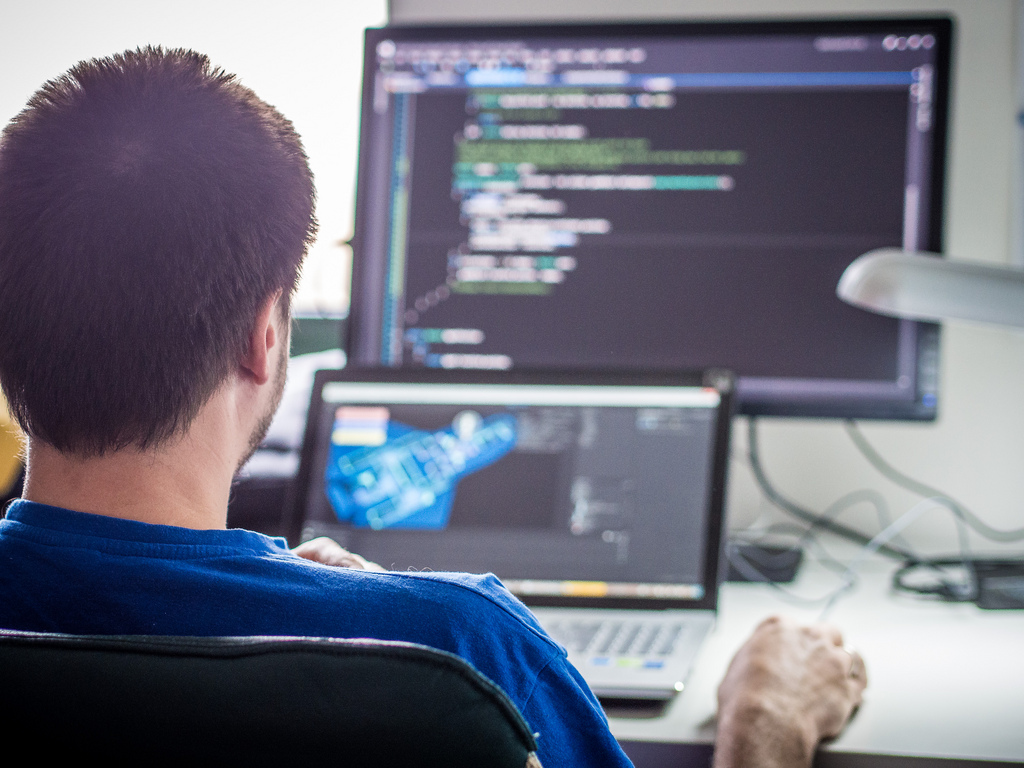
\includegraphics[width=13cm]{figs/programmer.jpg}}
% http://www.openweigh.com/assets/programmer-e898f9c9a43ecd208f1f1df347713e6e.jpg

\begin{frame}
\frametitle{Fundamentos de la asignatura}

\vspace{3.8cm}

\begin{center}
\color{red}
\Huge {\bf La programaci�n es el lenguaje de la tecnolog�a}
\end{center}

\end{frame}
\usebackgroundtemplate{}

%-----------------------    ---------------------------------

\begin{frame}
\frametitle{Lenguaje de Programaci�n: Python}

\begin{center}
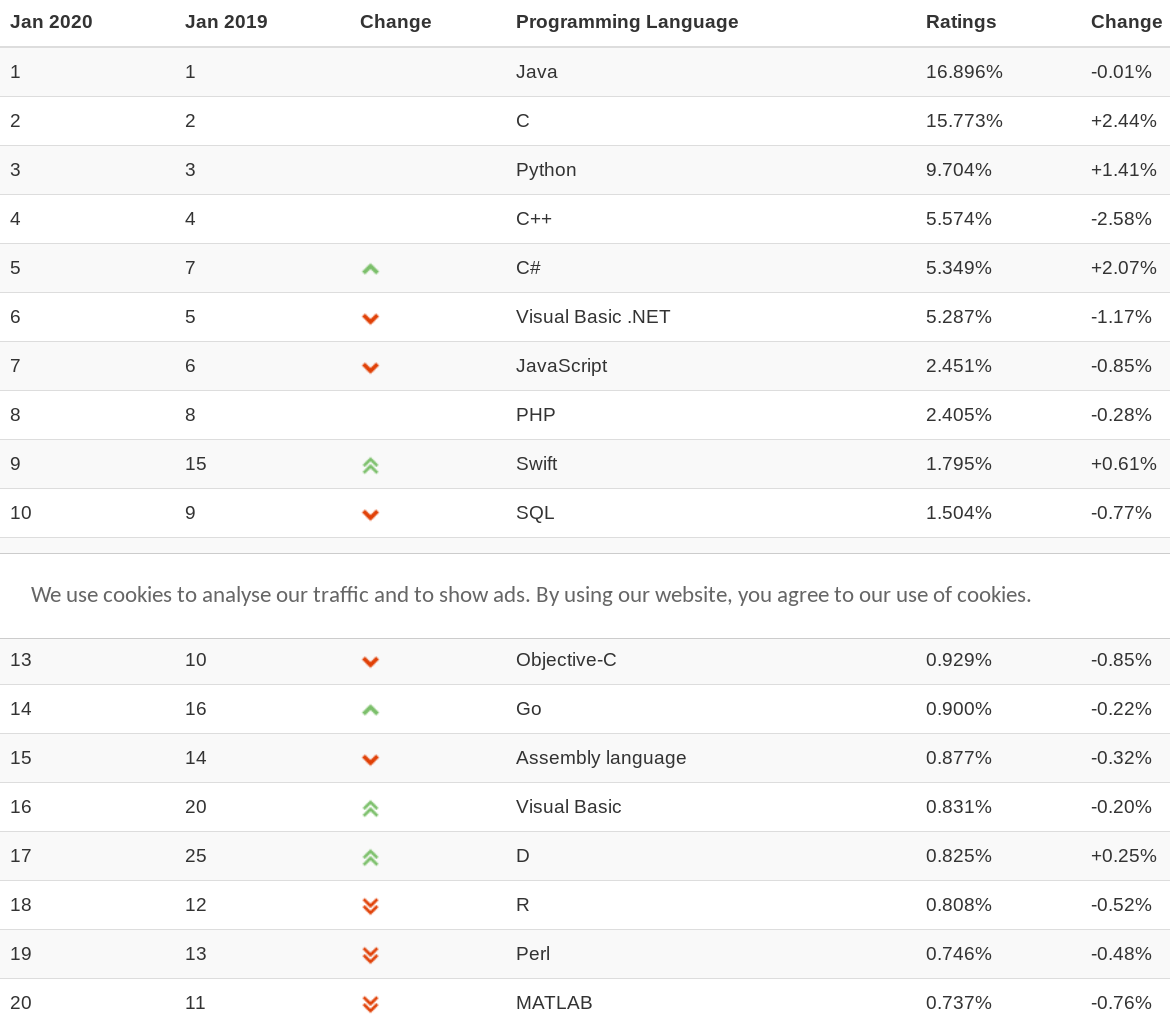
\includegraphics[width=5cm]{figs/2020-most-popular-lang-tiobe}
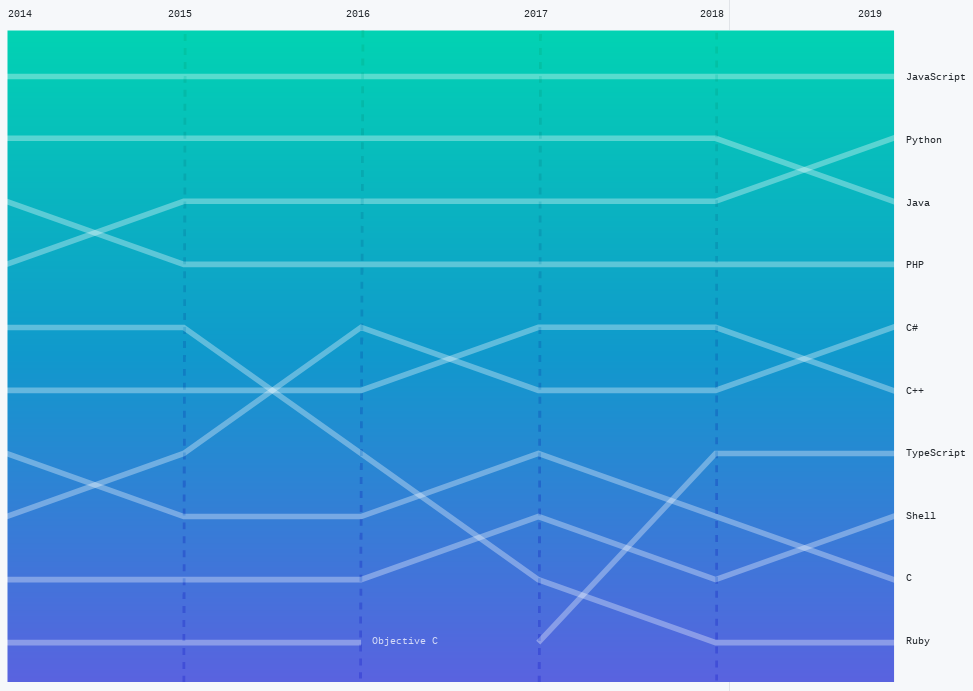
\includegraphics[width=6cm]{figs/2019-most-popular-lang-github}
\end{center}

\begin{center}
  {\Large Primer Mandamiento: \\ Amar�s Python por encima de (casi) todo.} \\
  TIOBE (enero 2020) ~~~~ GitHub (noviembre 2019) \\
\end{center}


\end{frame}
\usebackgroundtemplate{}


%-----------------------    ---------------------------------

\begin{frame}
\frametitle{Plataforma: Django}

\begin{center}
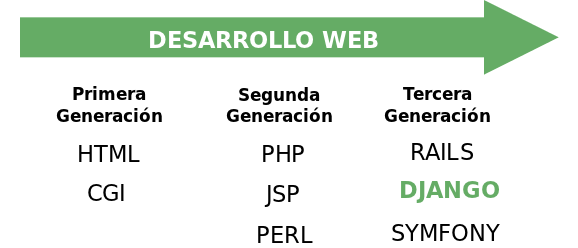
\includegraphics[width=11cm]{figs/django.png}
% http://www.maestrosdelweb.com/images/2012/04/desarrolloweb.png
\end{center}

\begin{center}
\Large Segundo Mandamiento: \\ No tomar�s el nombre de Django en vano.
\end{center}


\end{frame}
\usebackgroundtemplate{}

%%---------------------------------------------------------------

\begin{frame}
\frametitle{Metodolog�a}

{\Large
\begin{itemize}
\item Objetivo principal: conceptos b�sicos de construcci�n de sitios web modernos
\item Clases de teor�a y de pr�cticas, pero...
\item Teor�a en pr�cticas, pr�cticas en teor�a
\item Uso de resoluci�n de problemas para aprender
\item Fundamentalmente, entender lo fundamental
\end{itemize}
}
\end{frame}

%-----------------------    ---------------------------------
\usebackgroundtemplate{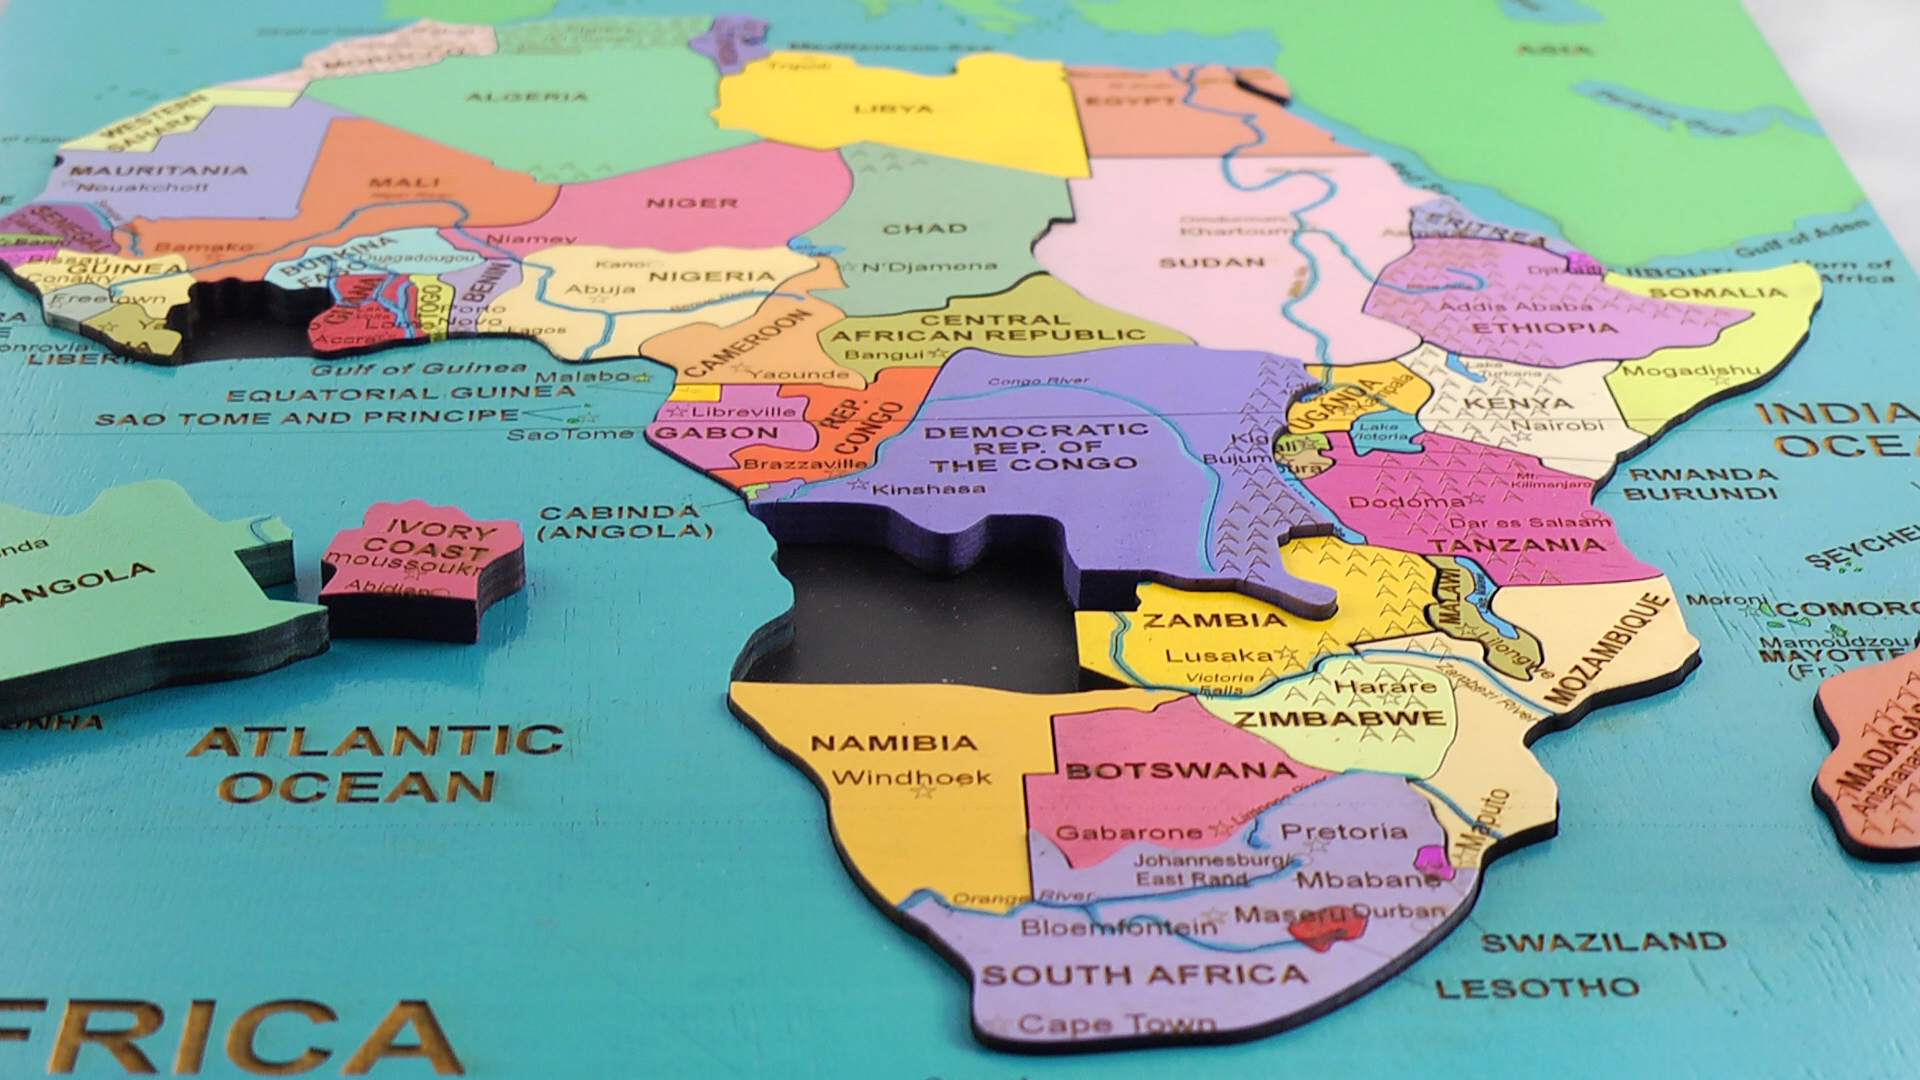
\includegraphics[width=13cm]{figs/africa.jpg}}
% http://www.funlearningcompany.com/wp-content/themes/smallbiz/images/Map100.jpg

\begin{frame}
\frametitle{Fundamentos de la asignatura}

\vspace{5.4cm}

\begin{center}
\Huge Aprender no puede ser aburrido
\end{center}

\end{frame}
\usebackgroundtemplate{}

%%---------------------------------------------------------------

\begin{frame}
\frametitle{Las Clases}

\begin{itemize}
  \item Empezamos en punto
  \item 10 minutos con un tema motivacional
  \begin{itemize}
    \item Gadgets tecnol�gicos
    \item Aplicaciones
    \item Cuestiones interesantes
    \item \dots
  \end{itemize}
  \item Generalmente, explicaci�n de los conceptos m�s importantes y luego
realizaci�n de ejercicios
  \item No hay descanso
  \item Ejercicios para hacer fuera de clase (y entregar)
\end{itemize}

\end{frame}



%-----------------------    ---------------------------------
\usebackgroundtemplate{
\includegraphics[width=13.5cm]{figs/challenge.jpg}}
% http://ichallenge.com/wp-content/uploads/2014/08/challenge-6.jpg

\begin{frame}
\frametitle{Fundamentos de la asignatura}

\vspace{-2.75cm}

\begin{center}
\Huge El estudiante es el centro del aprendizaje
\end{center}

\end{frame}
\usebackgroundtemplate{}



%%---------------------------------------------------------------

\begin{frame}
\frametitle{Evaluaci�n}

\begin{itemize}
\item Micropr�cticas diarias (entrega foro/GitLab): 0 a 1
\item Minipr�cticas preparatorias: 0 a 1
\item Pr�ctica final (obligatorio): 0 a 2.
\item Opciones y mejoras pr�ctica final: 0 a 3
\item Teor�a (obligatorio): 0 a 5.
\item Nota final: Suma de notas, moderada por la interpretaci�n del profesor
\item M�nimo para aprobar:
      \begin{itemize}
      \item Aprobado en teor�a (2.5) y pr�ctica final (1), y
      \item 5 puntos de nota final en total
      \end{itemize}
\end{itemize}

\end{frame}

%%---------------------------------------------------------------

\begin{frame}
\frametitle{Evaluaci�n (2)}

\begin{itemize}
\item Evaluaci�n teor�a: prueba escrita
\item Micropr�cticas diarias y minipr�cticas incrementales:
      \begin{itemize}
      \item es muy recomendable hacerlas
      \end{itemize}
\item Evaluaci�n pr�ctica final
      \begin{itemize}
      \item posibilidad de examen presencial para pr�ctica final
      \item �tiene que funcionar en el laboratorio!
      \item enunciado m�nimo obligatorio supone 1, se llega a 2 s�lo con calidad y cuidado en los detalles
      \end{itemize}
\item Opciones y mejoras pr�ctica final:
      \begin{itemize}
      \item permiten subir la nota mucho
      \end{itemize}
\item Evaluaci�n extraordinaria:
  \begin{itemize}
  \item prueba escrita (si no se aprob� la ordinaria)
  \item nueva pr�ctica final (si no se aprob� la ordinaria)
  \end{itemize}
\end{itemize}
\end{frame}


%%---------------------------------------------------------------

\begin{frame}
 \frametitle{Pr�cticas finales}

Ejemplos del pasado:

\begin{itemize}
 \item Servicio de b�squeda de hoteles
 \item Servicio de apoyo a la docencia
 \item Sitio de intercambio de fotos
 \item Aplicaci�n web de autoevaluaci�n docente
 \item Agregador de blogs (canales RSS)
 \item Agregador de microblogs (Identi.ca, Twitter)
\end{itemize}

\end{frame}



%%---------------------------------------------------------------

\begin{frame}
\frametitle{Ejemplos de pr�cticas finales de otros a�os}

\begin{itemize}
  \item Fernando Yustas: \url{https://www.youtube.com/watch?v=TUUMVEaBzeg}
  \item Miguel Ariza: \url{https://www.youtube.com/watch?v=fVBx9cGPjWs}
\end{itemize}

(puedes buscar en YouTube por muchos m�s ejemplos)

\end{frame}



%%---------------------------------------------------------------

\begin{frame}
\frametitle{��nimo!}

\begin{center}
{\huge Aqu� se ense�an c�mo son las cosas \\
  que se usan en el mundo real \\
  ~ \\
  Las buenas noticias son\dots \\
  que no son tan dif�ciles\\}
\end{center}

\end{frame}




%% $Id$
%


\section{HTML: HyperText Markup Language}

%%---------------------------------------------------------------

\begin{frame}[fragile]
\frametitle{Basic structure of a document}

\begin{verbatim}
<!DOCTYPE html>
<html>
 <head>
  <title> Tittle </title>
 </head>
 <body>
  <p>This is a paragraph</p>
 </body>
</html>
\end{verbatim}

\textbf{Ejercicio:} Escribe una p�gina HTML simple, y m�rala en el navegador.

\end{frame}


%%---------------------------------------------------------------

\begin{frame}[fragile]
\frametitle{Basic structure of a document (2)}

[Nota: en general, se describir� HTML5]

\begin{itemize}
\item \verb|<!DOCTYPE html>| es la marca de HTML5
\item En HTML 4.x era m�s complicado...
\item En general, cada elemento se abre y se cierra
\item La estructura de un documento es un �rbol \\
  (cada elemento va dentro de otro)
\item Elemento ra�z: HTML
\item Elementos bajo HTML: HEAD (indicaciones) y BODY (contenidos) 
\end{itemize}

\end{frame}

%%---------------------------------------------------------------

\begin{frame}[fragile]
\frametitle{Sintaxis b�sica}

Sintaxis similar a la de XML:

\begin{itemize}
\item Etiquetas (elementos, marcas): 
\begin{verbatim}
<p> ... </p> 
<p/>
\end{verbatim}

\item Atributos: 
\begin{verbatim}
<p id="abstract">
\end{verbatim}
\item Las etiquetas han de estar ``encapsuladas'': \\
  se cierran en orden inverso al que se abrieron \\
  (esto es, van siempre ``unas dentro de otras'', son contenedores)
\item Las etiquetas son nodos en el �rbol, \\
  los atributos anotaciones de los nodos
\item Caracteres ``escapados'': \verb|&lt;| ($<$) \verb|&gt;| ($>$)
\end{itemize}

\textbf{Ejercicio:} Escribe una p�gina HTML con cabecera (que tenga al menos un t�tulo) y cuerpo, con las dos sintaxis de etiquetas, y con elementos que tengan atributos.

\end{frame}

%%---------------------------------------------------------------

\begin{frame}[fragile]
\frametitle{Elemento HTML}

\begin{itemize}
\item Sintaxis b�sica:

\begin{verbatim}
<html lang="es">
\end{verbatim}

\item ``lang'' es el idioma (primario) del texto

\item Contiene un elemento HEAD y un elemento BODY
\end{itemize}

\begin{flushright}
Language tags in HTML and XML: \\
\url{http://www.w3.org/International/articles/language-tags/} \\
\end{flushright}
\end{frame}

%%---------------------------------------------------------------

\begin{frame}[fragile]
\frametitle{Elemento HEAD}

Informaci�n para el navegador y para bots.

Ejemplo:

\begin{verbatim}
<head>
  <meta charset="utf-8" />
  <title>El titulo</title>
  <link rel="stylesheet" type="text/css" href="main.css" />
  <link rel="alternate" type="application/atom+xml"
                        title="Canal RSS"
                        href="canal.rss" />
  <link rel="shortcut icon" href="/favicon.ico" />
</head>
\end{verbatim}

\end{frame}

\begin{frame}[fragile]
\frametitle{Elemento HEAD (2)}

\begin{itemize}
\item META:
  \begin{itemize}
  \item juego de caracteres \\
    (simplifica versiones pre-HTML5, \verb|http-equiv|)
  \item  description
  \end{itemize}
\item LINK puede apuntar a complementos para la p�gina
  \begin{itemize}
  \item rel="stylesheet": hoja de estilo CSS
  \end{itemize} 
\item LINK puede apuntar a otros recursos relacionados
  \begin{itemize}
  \item \verb|rel="alternate"|: contenido equivalente de otros tipos (type) \\
    o en otros idiomas (hreflang)
  \item \verb|rel="author"|: autor
  \item \verb|rel="next"|, \verb|rel="prev"|: anterior, posterior
  \item \verb|rel="shortcut icon"|: icono de la p�gina
  \item Otros: license, nofollow, search, tag, etc.
  \end{itemize} 
\item Otros: STYLE, SCRIPT (CSS o JavaScript embebidos)
\end{itemize}

\end{frame}

%%---------------------------------------------------------------

\begin{frame}[fragile]
\frametitle{Elementos en BODY}

\begin{itemize}
\item H1 - H6: cabeceras (headings)
\item P: parrafos de texto
\item A: ancla (anchor) (absoluto a url, absoluto a recurso, relativo)
\begin{verbatim}
<a href="http://linkedsite/url.html">Documento</a>
<a href="/url.html">Documento en mismo sitio</a>
<a href="url.html">Documento en mismo sitio y "dir"</a>
\end{verbatim}

\item UL, OL, DL: listas (sin ordenar, ordenadas, de definiciones)
\begin{verbatim}
<ul>
  <li>Un elemento</li>
  <li>Otro elemento</li>
</ul>
\end{verbatim}

\end{itemize}

\end{frame}

%%---------------------------------------------------------------

\begin{frame}[fragile]
\frametitle{Elementos en BODY (2)}

\begin{itemize}
\item Tabla
\begin{verbatim}
<table>
 <tr>
  <td>Primera fila, primera columna</td>
  <td>Primera fila, segunda columna</td>
 </tr>
 <tr>
  <td>Segunda fila, primera columna</td>
  <td>Segunda fila, segunda columna</td>
 </tr>
</table> 
\end{verbatim}

\end{itemize}

\end{frame}

%%---------------------------------------------------------------

\begin{frame}[fragile]
\frametitle{Elementos en BODY (3)}

\begin{itemize}
\item DIV: contenedor gen�rico (referncias para CSS)
\item HEADER, FOOTER, NAV, ARTICLE, SECTION, ASIDE: \\
  elementos de secci�n
\item IMG: im�genes
\begin{verbatim}
<img src="gsyc-bg.png" alt="Logo de GSyC">
<img src="gsyc-bg.png" alt="Logo de GSyC" width="300" height="240">
\end{verbatim}

\item MAP, AREA: mapa de imagen en el lado del cliente
\end{itemize}

\end{frame}

%%---------------------------------------------------------------

\begin{frame}[fragile]
\frametitle{Elementos en BODY (4)}

\begin{itemize}
\item FORM, FIELDSET, LABEL, INPUT

\begin{verbatim}
<form action="recurso" method="post">
  <fieldset>
    <legend>Formulario</legend>
 
    <label>Nombre</label>
    <input type="text" name="nombre"><br />
 
    <label>Apellido</label>
    <input type="text" name="apellido"><br />
 
    <input type="submit" name="persona">
 </fieldset>
</form>
\end{verbatim}

\end{itemize}
\end{frame}

%%---------------------------------------------------------------

\begin{frame}
\frametitle{Material complementario}

\begin{itemize}
\item HyperText Markup Language (Wikibook): \\
  \url{http://en.wikibooks.org/wiki/HTML_Programming}
\item HTML5: A tutorial for beginners: \\
  \url{http://www.html-5-tutorial.com/}
\item Dive into HTML5: \\
  \url{http://diveintohtml5.info}
\item HTML5 (Wikipedia): \\
  \url{http://en.wikipedia.org/wiki/HTML5}
\item Web Fundametals (Code Academy): \\
  \url{http://www.codecademy.com/tracks/web}
\end{itemize}


\end{frame}


%% $Id$
%

\section{Hojas de estilo CSS}


%%---------------------------------------------------------------

\begin{frame}
\frametitle{�Qu� es CSS?}

\begin{itemize}
  \item Es un lenguaje de hojas de estilos creado para {\bf controlar el aspecto} o presentaci�n de los documentos electr�nicos definidos con HTML
  \item Es la mejor forma de {\bf separar los contenidos y su presentaci�n} y es imprescindible para crear p�ginas web complejas
  \begin{itemize}
    \item Obliga a crear documentos HTML bien definidos y con significado completo (tambi�n llamados \emph{documentos sem�nticos})
    \item Mejora la accesibilidad del documento
    \item Reduce la complejidad de su mantenimiento
    \item Permite visualizar el mismo documento en infinidad de dispositivos diferentes
  \end{itemize}
\end{itemize}

\end{frame}

%%---------------------------------------------------------------

\begin{frame}[fragile]
\frametitle{Antes del CSS}

{\footnotesize
\begin{verbatim}
<!DOCTYPE html>
<html>
<head>
 <meta http-equiv="Content-Type" content="text/html; charset=iso-8859-1"/>
 <title>Ejemplo de estilos sin CSS</title>
</head>
 
<body>
 <h1><font color="red" face="Arial" size="5">
    Titular de la p�gina
 </font></h1>
 <p><font color="gray" face="Verdana" size="2">
   Un p�rrafo de texto no muy largo.
 </font></p>
</body>
</html>
\end{verbatim}
}

\end{frame}

%%---------------------------------------------------------------

\begin{frame}[fragile]
\frametitle{Con CSS}

{\footnotesize
\begin{verbatim}
<!DOCTYPE html">
<html>
<head>
<meta http-equiv="Content-Type" content="text/html; charset=iso-8859-1"/>
<title>Ejemplo de estilos con CSS</title>
<style type="text/css">
  h1 { color: red;  font-family: Arial;   font-size: large;  }
  p  { color: gray; font-family: Verdana; font-size: medium; }
</style>
</head>
 
<body>
  <h1>Titular de la p�gina</h1>
  <p>Un p�rrafo de texto no muy largo.</p>
</body>
</html>
\end{verbatim}
}

\end{frame}

%%---------------------------------------------------------------

\begin{frame}
\frametitle{CSS en un documento HTML}

Se pueden integrar instrucciones CSS de varias maneras en un documento
HTML:

\begin{enumerate}
  \item Incluir CSS en el mismo documento HTML
  \item Definir CSS en un archivo externo
  \item Incluir CSS en los elementos HTML
\end{enumerate}

\end{frame}

%%---------------------------------------------------------------

\begin{frame}
\frametitle{Glosario B�sico (I)}

\begin{center}
\begin{figure}[p]
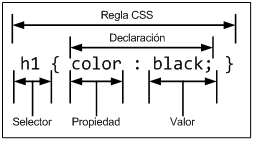
\includegraphics[width=0.6\textwidth]{figs/f0101.png}
\end{figure}
\end{center}

\begin{itemize}
  \item {\bf Regla}: cada uno de los estilos que componen una hoja de estilos CSS. Cada regla est� compuesta de una parte de ``selectores'', un s�mbolo de ``llave de apertura'' (\{), otra parte denominada ``declaraci�n'' y por �ltimo, un s�mbolo de ``llave de cierre'' (\}).
  \item {\bf Selector}: indica el elemento o elementos HTML a los que se aplica la regla CSS.
\end{itemize}

\end{frame}

%%---------------------------------------------------------------

\begin{frame}
\frametitle{Glosario B�sico (y II)}

\begin{center}
\begin{figure}[p]
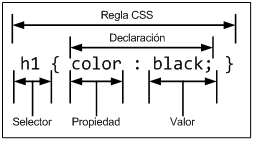
\includegraphics[width=0.42\textwidth]{figs/f0101.png}
\end{figure}
\end{center}

\begin{itemize}
  \item {\bf Declaraci�n}: especifica los estilos que se aplican a los elementos. Est� compuesta por una o m�s propiedades CSS.
  \item {\bf Propiedad}: caracter�stica que se modifica en el elemento seleccionado, como por ejemplo su tama�o de letra, su color de fondo, etc.
  \item {\bf Valor}: establece el nuevo valor de la caracter�stica modificada en el elemento.
\end{itemize}

CSS 2.1 define 115 propiedades, mientras que CSS 3 define 239 propiedades.

\end{frame}

%%---------------------------------------------------------------
%
%\begin{frame}
%\frametitle{Sintaxis}
%
%\begin{itemize}
%  \item Sucesi�n de palabras sin ning�n car�cter que las separe (par�ntesis, comas, barras, etc.) el valor de la propiedad se debe indicar tal y como se muestra y con esas palabras en el mismo orden.
%  \item Sucesi�n de valores separados por una barra simple el valor de la propiedad debe tomar uno y s�lo uno de los valores indicados
%  \item Sucesi�n de valores separados por una barra doble el valor de la propiedad puede tomar uno o m�s valores de los indicados y en cualquier orden.
%  \item Cada valor o agrupaci�n de valores se puede indicar el tipo de valor: opcional, obligatorio, m�ltiple o restringido.
%  \item M�s: * = cero o m�s veces; + = una o m�s veces; ? = opcional; {n1, n2} = entre n1 y n2 veces
%\end{itemize}
%
%\end{frame}


%%---------------------------------------------------------------

\subsubsection*{Selectores}

\begin{frame}
\frametitle{Selectores}

\begin{itemize}
  \item A un mismo elemento HTML se le pueden aplicar varias reglas 
  \item Cada regla puede aplicarse a un n�mero ilimitado de elementos
  \item Cuando el selector de dos o m�s reglas CSS es id�ntico, se pueden agrupar las declaraciones de las reglas para hacer las hojas de estilos m�s eficientes
  \item Cuando se establece el valor de una propiedad CSS en un elemento, sus elementos descendientes heredan de forma autom�tica el valor de esa propiedad
\end{itemize}

CSS 2.1 incluye una docena de tipos diferentes de selectores, que permiten seleccionar de forma muy precisa elementos individuales o conjuntos de elementos dentro de una p�gina web.

\end{frame}

%%---------------------------------------------------------------

\begin{frame}
\frametitle{Selectores b�sicos}

\begin{enumerate}
  \item Selector universal
  \item Selector de tipo o etiqueta
  \item Selector descendente
  \item Selector de clase
  \item Selector de identidad
\end{enumerate}

\end{frame}

%%---------------------------------------------------------------

\begin{frame}[fragile]
\frametitle{Selector Universal}

\begin{itemize}
  \item No se utiliza habitualmente
  \item Generalmente es equivalente para poner estilo a $<body>$
  \item Se suele combinar con otros selectores y adem�s, forma parte de algunos hacks muy utilizados
\end{itemize}

\begin{verbatim}
* {
  margin: 0;
  padding: 0;
}
\end{verbatim}

\end{frame}

%%---------------------------------------------------------------

\begin{frame}[fragile]
\frametitle{Selector de tipo o etiqueta}

\begin{itemize}
  \item Selecciona todos los elementos de la p�gina cuya etiqueta HTML coincide con el valor del selector
  \item Se pueden agrupar todas las reglas individuales en una sola regla con un selector m�ltiple.
  \item Buena pr�ctica: agrupar las propiedades comunes de varios elementos en una �nica regla CSS y posteriormente definir las propiedades espec�ficas de esos mismos elementos
\end{itemize}

{\footnotesize
\begin{verbatim}
h1, h2, h3 {
  color: #8A8E27;
  font-weight: normal;
  font-family: Arial, Helvetica, sans-serif;
}
 
h1 { font-size: 2em; }
h2 { font-size: 1.5em; }
h3 { font-size: 1.2em; }
\end{verbatim}
}

\end{frame}

%%---------------------------------------------------------------

\begin{frame}[fragile]
\frametitle{Selector descendente}

\begin{itemize}
  \item Selecciona los elementos que se encuentran dentro de otros elementos. Un elemento es descendiente de otro cuando se encuentra entre las etiquetas de apertura y de cierre del otro elemento.
\end{itemize}

\begin{verbatim}
p span { color: red; }
[...]
<p>
  ...
  <span>texto1</span>
  ...
  <a href="">...<span>texto2</span></a>
  ...
</p>
\end{verbatim}

Al resto de elementos $<span>$ de la p�gina que no est�n dentro de un elemento $<p>$, no se les aplica la regla CSS anterior.

\end{frame}

%%---------------------------------------------------------------

\begin{frame}
\frametitle{Ejercicio}

�Qu� elementos se seleccionar�an con estos tipos de selectores?

\begin{itemize}
  \item p a span em \{ text-decoration: underline; \}
  \item p, a, span, em \{ text-decoration: underline; \}
  \item p a \{ color: red; \}
  \item p * a \{ color: red; \}
\end{itemize}

\end{frame}

%%---------------------------------------------------------------

\begin{frame}[fragile]
\frametitle{Selector de clase}

\begin{itemize}
  \item Se utiliza el atributo class de HTML sobre ese elemento para indicar directamente la regla CSS que se le debe aplicar
  \item Se crea en el archivo CSS una nueva regla llamada destacado con todos los estilos que se van a aplicar al elemento
  \item Se prefija el valor del atributo class con un punto (.)
\end{itemize}

{\footnotesize
\begin{verbatim}
.destacado { color: red; }
[...]
  <p class="destacado">Lorem ipsum dolor sit amet...</p>
  <p>Nunc sed lacus et 
<a href="#" class="destacado">est adipiscing</a>
  accumsan...</p>
  <p>Class aptent taciti <em class="destacado">sociosqu
ad</em> litora...</p>
\end{verbatim}
}

\end{frame}

%%---------------------------------------------------------------

\begin{frame}[fragile]
\frametitle{Selector de clase m�s espec�fico}

\begin{itemize}
  \item Combinando el selector de tipo y el selector de clase, se obtiene un selector mucho m�s espec�fico.
\end{itemize}

{\footnotesize
\begin{verbatim}
p.destacado { color: red }
[...]
  <p class="destacado">Lorem ipsum dolor sit amet...</p>
  <p>Nunc sed lacus et <a href="#" class="destacado">est
adipiscing</a> accumsan...</p>
  <p>Class aptent taciti <em class="destacado">sociosqu
ad</em> litora...</p>
\end{verbatim}
}

\end{frame}

%%---------------------------------------------------------------

\begin{frame}
\frametitle{Ejercicio}

�Qu� elementos se seleccionar�an con estos tipos de selectores?

\begin{itemize}
  \item p.aviso \{ ... \}
  \item p .aviso \{ ... \}
  \item p, .aviso \{ ... \}
  \item *.aviso \{ ... \}
\end{itemize}

\end{frame}

%%---------------------------------------------------------------

\begin{frame}[fragile]
\frametitle{Selectores de identificador}

\begin{itemize}
  \item Aplica estilos CSS a un �nico elemento de la p�gina
  \item El valor del atributo id no se puede repetir en dos elementos diferentes de una misma p�gina
\end{itemize}

\begin{verbatim}
#destacado { color: red; }
 
<p>Primer p�rrafo</p>
<p id="destacado">Segundo p�rrafo</p>
<p>Tercer p�rrafo</p>
\end{verbatim}

\end{frame}


%%---------------------------------------------------------------

\begin{frame}
\frametitle{Ejercicio}

�Qu� elementos se seleccionar�an con estos tipos de selectores?

\begin{itemize}
  \item p\#aviso \{ ... \}
  \item p \#aviso \{ ... \}
  \item p, \#aviso \{ ... \}
  \item *\#aviso \{ ... \}
\end{itemize}

�Tienen sentido estos selectores? �Cu�ndo?

\end{frame}

%%---------------------------------------------------------------

\begin{frame}
\frametitle{Ejercicio: Combinaci�n de selectores}

�Qu� elementos se seleccionar�an con estos tipos de selectores?

\begin{itemize}
  \item .aviso .especial \{ ... \}
  \item div.aviso span.especial \{ ... \}
  \item ul\#menuPrincipal li.destacado a\#inicio \{ ... \}
\end{itemize}

\end{frame}

%%---------------------------------------------------------------

\begin{frame}
\frametitle{Colisi�n de estilos (simplificado)}

\begin{enumerate}
  \item Cuanto m�s espec�fico sea un selector, m�s importancia tiene su regla asociada.
  \item A igual especificidad, se considera la �ltima regla indicada.
\end{enumerate}

\end{frame}



%%---------------------------------------------------------------

\subsubsection*{Unidades y colores}

\begin{frame}
\frametitle{Unidades de medida}

\begin{itemize}
  \item Unidades absolutas
  \begin{itemize}
    \item in, cm, mm, pt, pc
  \end{itemize}
  \item Unidades relativas
  \begin{itemize}
    \item em, ex, px
  \end{itemize}
  \item Porcentajes
\end{itemize}

En general, se recomienda el uso de unidades relativas siempre que sea posible

Normalmente se utilizan p�xel y porcentajes para definir el layout del documento (b�sicamente, la anchura de las columnas y de los elementos de las p�ginas) y em y porcentajes para el tama�o de letra de los textos.

\end{frame}

%%---------------------------------------------------------------

\begin{frame}
\frametitle{Colores}

\begin{itemize}
  \item Palabras clave
  \begin{itemize}
    \item aqua, black, blue, fuchsia, gray...
  \end{itemize}
  \item RGB decimal
  \item RGB porcentual
  \item RGB hexadecimal
\end{itemize}

\end{frame}


%%---------------------------------------------------------------

\begin{frame}
\frametitle{Tipos de elementos (I)}

El est�ndar HTML clasifica a todos sus elementos en dos grandes grupos:

Elementos de l�nea:

\begin{itemize}
  \item Los elementos en l�nea (``inline elements'' en ingl�s) no empiezan necesariamente en nueva l�nea y s�lo ocupan el espacio necesario para mostrar sus contenidos.

\end{itemize}

\end{frame}

%%---------------------------------------------------------------

\begin{frame}
\frametitle{Tipos de elementos (II)}

Elementos de bloque:

\begin{itemize}
  \item Los elementos de bloque (``block elements'' en ingl�s) siempre empiezan en una nueva l�nea y ocupan todo el espacio disponible hasta el final de la l�nea
\end{itemize}

\begin{center}
\begin{figure}[p]
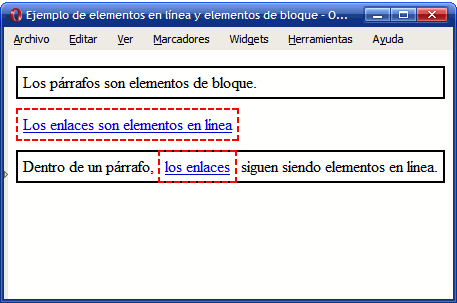
\includegraphics[width=0.8\textwidth]{figs/f0501.png}
\end{figure}
\end{center}

Por sus caracter�sticas, los elementos de bloque no pueden insertarse dentro de elementos en l�nea y tan s�lo pueden aparecer dentro de otros elementos de bloque. En cambio, un elemento en l�nea puede aparecer tanto dentro de un elemento de bloque como dentro de otro elemento en l�nea.

\end{frame}



%%---------------------------------------------------------------

\subsubsection*{El Modelo de Cajas}

\begin{frame}
\frametitle{El modelo de cajas}

\begin{itemize}
  \item Es el comportamiento de CSS que hace que todos los elementos de las p�ginas se representen mediante cajas rectangulares
  \item  Cada vez que se inserta una etiqueta HTML, se crea una nueva caja rectangular que encierra los contenidos de ese elemento
\end{itemize}


\begin{center}
\begin{figure}[p]
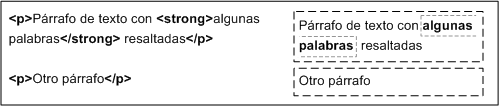
\includegraphics[width=0.8\textwidth]{figs/f0402.png}
\end{figure}
\end{center}

\end{frame}

%%---------------------------------------------------------------

\begin{frame}
\frametitle{El modelo de cajas (II)}

\begin{itemize}
  \item No son visibles a simple vista porque inicialmente no muestran ning�n color de fondo ni ning�n borde
\end{itemize}

\begin{center}
\begin{figure}[p]
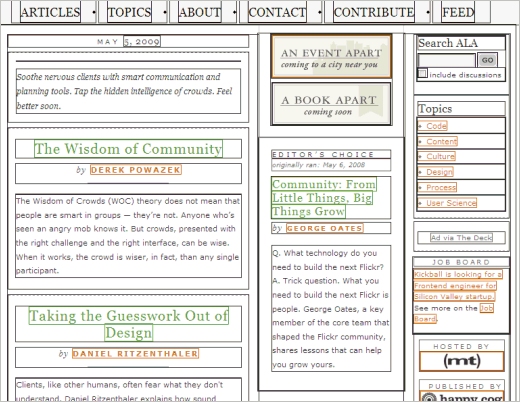
\includegraphics[width=0.55\textwidth]{figs/f0401.png}
\end{figure}
\end{center}
{\footnotesize
Ejemplo de http://www.alistapart.com/ despu�s de forzar a que todas las cajas muestren su borde
}

\end{frame}

%%---------------------------------------------------------------

\begin{frame}
\frametitle{El modelo de cajas (III)}

\begin{itemize}
  \item Los navegadores crean y colocan las cajas de forma autom�tica, pero CSS permite modificar todas sus caracter�sticas. Cada una de las cajas est� formada por seis partes, tal y como muestra la siguiente imagen:
\end{itemize}


\begin{center}
\begin{figure}[p]
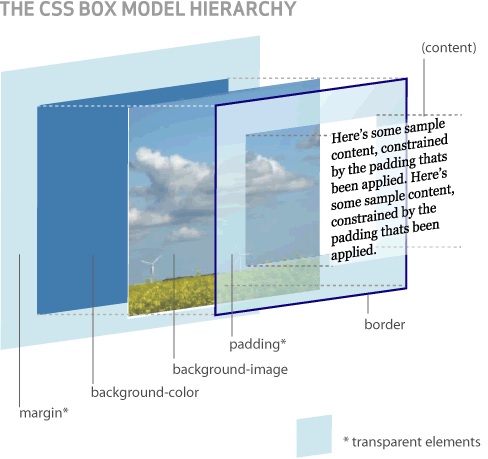
\includegraphics[width=0.45\textwidth]{figs/f0403.png}
\end{figure}
\end{center}
{\footnotesize
 Representaci�n tridimensional del box model de CSS
(Esquema utilizado con permiso de http://www.hicksdesign.co.uk/boxmodel/)
}
\end{frame}

%%---------------------------------------------------------------

\begin{frame}
\frametitle{Partes que componen cada caja}

\begin{itemize}
  \item {\bf Contenido} (content): se trata del contenido HTML del elemento (las palabras de un p�rrafo, una imagen, el texto de una lista de elementos, etc.)
  \item {\bf Relleno} (padding): espacio libre opcional existente entre el contenido y el borde.
  \item {\bf Borde} (border): l�nea que encierra completamente el contenido y su relleno.
  \item {\bf Imagen de fondo} (background image): imagen que se muestra por detr�s del contenido y el espacio de relleno.
  \item {\bf Color de fondo} (background color): color que se muestra por detr�s del contenido y el espacio de relleno.
  \item {\bf Margen} (margin): separaci�n opcional existente entre la caja y el resto de cajas adyacentes.
\end{itemize}

\end{frame}


%%---------------------------------------------------------------

\begin{frame}[fragile]
\frametitle{Margen, relleno, bordes y modelo de cajas (I)}

\begin{itemize}
  \item El margen, el relleno y los bordes establecidos a un elemento determinan la anchura y altura final del elemento
\end{itemize}

{\footnotesize
\begin{verbatim}
div {
  width: 300px;
  padding-left:  50px;
  padding-right: 50px;
  margin-left:   30px;
  margin-right:  30px;
  border: 10px solid black;
}
\end{verbatim}
}



\end{frame}

%%---------------------------------------------------------------

\begin{frame}[fragile]
\frametitle{Margen, relleno, bordes y modelo de cajas (y II)}

\begin{center}
\begin{figure}[p]
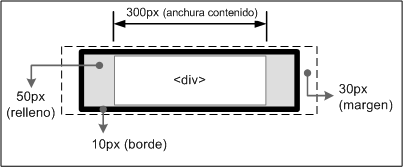
\includegraphics[width=0.75\textwidth]{figs/f0414.png}
\end{figure}
\end{center}

De esta forma, la anchura del elemento en pantalla ser�a igual a la suma de la anchura original, los m�rgenes, los bordes y los rellenos:

30px + 10px + 50px + 300px + 50px + 10px + 30px = 480 p�xel

\end{frame}

%%---------------------------------------------------------------

\begin{frame}
\frametitle{Visualizaci�n}

\begin{itemize}
  \item CSS define otras cuatro propiedades para controlar su visualizaci�n: display, visibility, overflow y z-index.
  \item La propiedad display permite ocultar completamente un elemento haciendo que desaparezca de la p�gina. Como el elemento oculto no se muestra, el resto de elementos de la p�gina se mueven para ocupar su lugar.
  \item La propiedad display tambi�n permite modificar el comportamiento de un elemento a bloque (block) o en l�nea (inline).
  \item La propiedad visibility permite hacer invisible un elemento, lo que significa que el navegador crea la caja del elemento pero no la muestra. En este caso, el resto de elementos de la p�gina no modifican su posici�n, ya que aunque la caja no se ve, sigue ocupando sitio.
\end{itemize}

\end{frame}


%%---------------------------------------------------------------

\begin{frame}
\frametitle{Diferencias entre display y visibility}

\begin{center}
\begin{figure}[p]
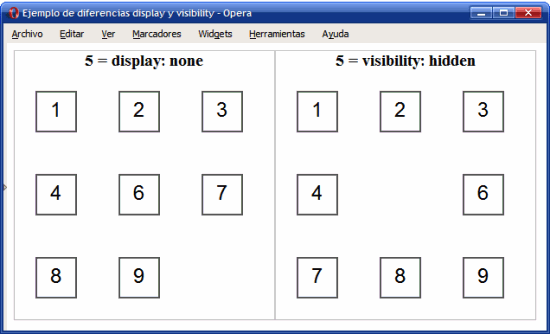
\includegraphics[width=0.8\textwidth]{figs/f0522.png}
\end{figure}
\end{center}

\end{frame}



%%---------------------------------------------------------------

\begin{frame}
\frametitle{Propiedades margin}

\begin{center}
  \begin{table}
   \begin{tabular}{p{1.8cm}p{7.8cm}}
Propiedades &\bf{margin-top}, \bf{margin-right}, \bf{margin-bottom}, \bf{margin-left} \\ \hline
Valores & $<medida>$ | $<porcentaje>$ | auto | inherit \\ \hline
Se aplica a & Todos los elementos, salvo margin-top y margin-bottom que s�lo se aplican a los elementos de bloque y a las im�genes \\ \hline
Valor inicial & 0 \\ \hline
Descripci�n & Establece cada uno de los m�rgenes horizontales y verticales de un elemento \\  \hline
  \end{tabular}
    \caption{Definici�n de la propiedad \emph{margin-top}, \emph{margin-right}, \emph{margin-bottom}, \emph{margin-left} de CSS}
 \end{table}
\end{center}

\end{frame}

%%---------------------------------------------------------------

\begin{frame}
\frametitle{Propiedad margin (propiedad \emph{shorthand})}

\begin{center}
  \begin{table}
   \begin{tabular}{p{1.8cm}p{7.8cm}}
Propiedad &\bf{margin} \\ \hline
Valores & ( $<medida>$ | $<porcentaje>$ | auto ) {1, 4} | inherit \\ \hline
Se aplica a & Todos los elementos salvo algunos casos especiales de elementos mostrados como tablas \\ \hline
Valor inicial & - \\ \hline
Descripci�n & Establece de forma directa todos los m�rgenes de un elemento \\ \hline
 \end{tabular}
   \caption{Definici�n de la propiedad margin de CSS}
 \end{table}
\end{center}

\end{frame}

%%---------------------------------------------------------------

\begin{frame}
\frametitle{Propiedad margin (propiedad \emph{shorthand}) (y II)}

La notaci�n {1, 4} de la definici�n anterior significa que la propiedad margin admite entre uno y cuatro valores, con el siguiente significado:

\begin{itemize}
  \item Si solo se indica un valor, todos los m�rgenes tienen ese valor.
  \item Si se indican dos valores, el primero se asigna al margen superior e inferior y el segundo se asigna a los m�rgenes izquierdo y derecho.
  \item Si se indican tres valores, el primero se asigna al margen superior, el tercero se asigna al margen inferior y el segundo valor se asigna los m�rgenes izquierdo y derecho.
  \item Si se indican los cuatro valores, el orden de asignaci�n es: margen superior, margen derecho, margen inferior y margen izquierdo.
\end{itemize}

\end{frame}


\begin{frame}
\frametitle{Posicionamiento y visualizaci�n}

\begin{itemize}
  \item Los navegadores crean y posicionan de forma autom�tica todas las cajas que forman cada p�gina HTML
  \item El dise�ador puede modificar la posici�n en la que se muestra cada caja.
  \item Existen {\bf cuatro tipos de posicionamiento} definidos para las cajas
\end{itemize}

\end{frame}



%%---------------------------------------------------------------

\begin{frame}
\frametitle{Tipos de posicionamiento}

\begin{itemize}
  \item {\bf Normal o est�tico}: posicionamientosi no se indica lo contrario.
  \item{\bf Relativo}: consiste en posicionar una caja seg�n el posicionamiento normal y despu�s desplazarla respecto de su posici�n original.
  \item {\bf Absoluto}: la posici�n de una caja se establece de forma absoluta respecto de su elemento contenedor y el resto de elementos de la p�gina ignoran la nueva posici�n del elemento.
  \item {\bf Fijo}: variante del posicionamiento absoluto que convierte una caja en un elemento inamovible, de forma que su posici�n en la pantalla siempre es la misma independientemente del resto de elementos e independientemente de si el usuario sube o baja la p�gina en la ventana del navegador.
  \item {\bf Flotante}: desplaza las cajas todo lo posible hacia la izquierda o hacia la derecha de la l�nea en la que se encuentran.
\end{itemize}

\end{frame}

%%---------------------------------------------------------------
\subsubsection*{Enlaces}

\begin{frame}
\frametitle{Pseudo-clases}

Como con los atributos id o class no es posible aplicar diferentes estilos a un mismo elemento en funci�n de su estado, CSS introduce un nuevo concepto llamado pseudo-clases. En enlaces:

\begin{itemize}
  \item {\bf :link}: enlaces que apuntan a p�ginas o recursos que a�n no han sido visitados por el usuario.
  \item {\bf :visited}: enlaces que apuntan a recursos que han sido visitados anteriormente por el usuario. El historial de enlaces visitados se borra autom�ticamente cada cierto tiempo y el usuario tambi�n puede borrarlo manualmente.
  \item {\bf :hover}: enlace sobre el que el usuario ha posicionado el puntero del rat�n.
  \item {\bf :active}: enlace que est� pinchando el usuario. Los estilos s�lo se aplican desde que el usuario pincha el bot�n del rat�n hasta que lo suelta.
\end{itemize}

\end{frame}


%%---------------------------------------------------------------

\begin{frame}
\frametitle{Im�genes seg�n el estilo del enlace}

\begin{itemize}
  \item En ocasiones, puede resultar �til incluir un peque�o icono al lado de un enlace para indicar el tipo de contenido que enlaza.
  \item Este tipo de im�genes son puramente decorativas en vez de im�genes de contenido, por lo que se deber�an a�adir con CSS y no con elementos de tipo $<img>$. Utilizando la propiedad background (y background-image) se puede personalizar el aspecto de los enlaces para que incluyan un peque�o icono a su lado.
  \item La t�cnica consiste en mostrar una imagen de fondo sin repetici�n en el enlace y a�adir el padding necesario al texto del enlace para que no se solape con la imagen de fondo.
\end{itemize}

\end{frame}


%%---------------------------------------------------------------

\begin{frame}[fragile]
\frametitle{Im�genes seg�n el estilo del enlace (II)}

\begin{footnotesize}
\begin{verbatim}
a { margin: 1em 0; float: left; clear: left; }
 
.rss {
  color: #E37529;
  padding: 0 0 0 18px;
  background: #FFF url(imagenes/rss.gif) no-repeat left center;
}
 
.pdf {
  padding: 0 0 0 22px;
  background: #FFF url(imagenes/pdf.png) no-repeat left center;
}
 
<a href="#">Enlace con el estilo por defecto</a>
<a class="rss" href="#">Enlace a un archivo RSS</a>
<a class="pdf" href="#">Enlace a un documento PDF</a>
\end{verbatim}
\end{footnotesize}

\end{frame}

%%---------------------------------------------------------------

\begin{frame}
\frametitle{Im�genes seg�n el estilo del enlace (y III)}


\begin{center}
\begin{figure}[p]
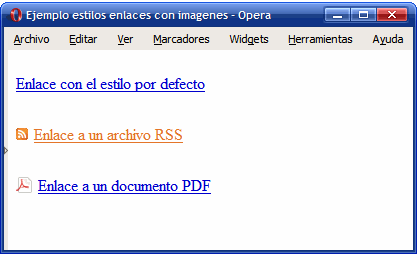
\includegraphics[width=0.8\textwidth]{figs/f0704.png}
\end{figure}
\end{center}

\end{frame}


%%---------------------------------------------------------------

\begin{frame}[fragile]
\frametitle{Mostrar los enlaces como si fueran botones}

\begin{footnotesize}
\begin{verbatim}
a { margin: 1em 0; float: left; clear: left; }
a.boton {
  text-decoration: none;
  background: #EEE;
  color: #222;
  border: 1px outset #CCC;
  padding: .1em .5em;
}
a.boton:hover {
  background: #CCB;
}
a.boton:active {
  border: 1px inset #000;
}
<a class="boton" href="#">Guardar</a>
<a class="boton" href="#">Enviar</a>
\end{verbatim}
\end{footnotesize}

\end{frame}



%%---------------------------------------------------------------

\begin{frame}
\frametitle{Crear un men� vertical}

\begin{enumerate}
  \item Definir anchura del men�
  \item Eliminar las vi�etas autom�ticas y todos los m�rgenes y espaciados aplicados por defecto
  \item A�adir un borde al men� de navegaci�n y establecer el color de fondo y los bordes de cada elemento del men�
  \item Aplicar estilos a los enlaces: mostrarlos como un elemento de bloque para que ocupen todo el espacio de cada $<$li> del men�, a�adir un espacio de relleno y modificar los colores y la decoraci�n por defecto
\end{enumerate}


\begin{center}
\begin{figure}[p]
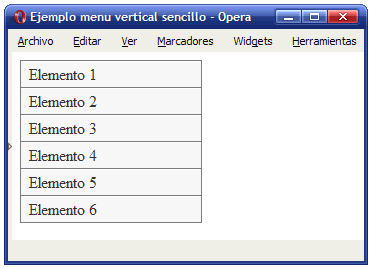
\includegraphics[width=0.6\textwidth]{figs/f0908.png}
\end{figure}
\end{center}

\end{frame}


%%---------------------------------------------------------------

\begin{frame}
\frametitle{Men� horizontal b�sico}

\begin{enumerate}
  \item Aplicar los estilos CSS b�sicos para establecer el estilo del men� (similares a los del men� vertical)
  \item  Establecer la anchura de los elementos del men�. Si el men� es de anchura variable y contiene cinco elementos, se asigna una anchura del 20\% a cada elemento
  \item Establecer los bordes de los elementos que forman el men�
  \item Se elimina el borde derecho del �ltimo elemento de la lista, para evitar el borde duplicado
\end{enumerate}


\begin{center}
\begin{figure}[p]
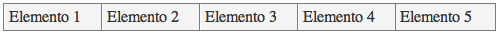
\includegraphics[width=0.8\textwidth]{figs/f0909.png}
\end{figure}
\end{center}

\end{frame}



%%---------------------------------------------------------------
%%---------------------------------------------------------------



\subsection*{CSS: Consideraciones adicionales}

\begin{frame}[fragile]
\frametitle{CSS: Consideraciones adicionales}

\begin{center}
{\Huge CSS \\ Consideraciones Adicionales}

{\footnotesize (transparencias de referencia)}

\end{center}


\end{frame}


%%---------------------------------------------------------------


\begin{frame}
\frametitle{Orden de visualizaci�n}

\begin{itemize}
  \item El relleno y el margen son transparentes, por lo que en el espacio ocupado por el relleno se muestra el color o imagen de fondo (si est�n definidos)
  \item En el espacio ocupado por el margen se muestra el color o imagen de fondo de su elemento padre (si est�n definidos)
  \item Si ning�n elemento padre tiene definido un color o imagen de fondo, se muestra el color o imagen de fondo de la propia p�gina (si est�n definidos)
  \item Si una caja define tanto un color como una imagen de fondo, la imagen tiene m�s prioridad y es la que se visualiza
  \item Si la imagen de fondo no cubre totalmente la caja del elemento o si la imagen tiene zonas transparentes, tambi�n se visualiza el color de fondo. 
\end{itemize}

\end{frame}



%%---------------------------------------------------------------

\begin{frame}
\frametitle{Propiedad width}

\begin{center}
  \begin{table}
   \begin{tabular}{p{1.8cm}p{7.8cm}}
Propiedad &\bf{width} \\ \hline
Valores & $<medida>$ | $<porcentaje>$ | auto | inherit \\ \hline
Se aplica a & Todos los elementos, salvo los elementos en l�nea que no sean im�genes, las filas de tabla y los grupos de filas de tabla \\ \hline
Valor inicial & auto \\ \hline
Descripci�n & Establece la anchura de un elemento \\ \hline
  \end{tabular}
   \caption{Definici�n de la propiedad \emph{width} de CSS}
 \end{table}
\end{center}

\end{frame}

%%---------------------------------------------------------------

\begin{frame}
\frametitle{Propiedad height}

\begin{center}
  \begin{table}
   \begin{tabular}{p{1.8cm}p{7.8cm}}
Propiedad &\bf{height} \\ \hline
Valores & $<medida>$ | $<porcentaje>$ | auto | inherit \\ \hline
Se aplica a & Todos los elementos, salvo los elementos en l�nea que no sean im�genes, las columnas de tabla y los grupos de columnas de tabla \\ \hline
Valor inicial & auto \\ \hline
Descripci�n & Establece la altura de un elemento \\ \hline
  \end{tabular}
   \caption{Definici�n de la propiedad \emph{height} de CSS}
 \end{table}
\end{center}

\end{frame}

%%---------------------------------------------------------------


\begin{frame}
\frametitle{M�rgenes}


\begin{center}
\begin{figure}[p]
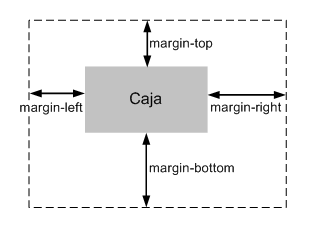
\includegraphics[width=0.45\textwidth]{figs/f0428.png}
\end{figure}
\end{center}

\begin{itemize}
  \item En vez de utilizar la etiqueta $<blockquote>$ de HTML, deber�a utilizarse la propiedad margin-left de CS
  \item Los m�rgenes verticales (margin-top y margin-bottom) s�lo se pueden aplicar a los elementos de bloque y las im�genes, mientras que los m�rgenes laterales (margin-left y margin-right) se pueden aplicar a cualquier elemento
\end{itemize}

\end{frame}


%%---------------------------------------------------------------

\begin{frame}
\frametitle{El margen vertical}

Es algo peculiar:

\begin{itemize}
  \item Cuando se juntan dos o m�s m�rgenes verticales, se fusionan de forma autom�tica y la altura del nuevo margen ser� igual a la altura del margen m�s alto de los que se han fusionado.
  \item Si un elemento est� contenido dentro de otro elemento, sus m�rgenes verticales se fusionan y resultan en un nuevo margen de la misma altura que el mayor margen de los que se han fusionado
  \item Si no se diera este comportamiento y se estableciera un determinado margen a todos los p�rrafos, el primer p�rrafo no mostrar�a un aspecto homog�neo respecto de los dem�s.
\end{itemize}

\end{frame}

%%---------------------------------------------------------------

\begin{frame}
\frametitle{Relleno}

\begin{center}
  \begin{table}
   \begin{tabular}{p{1.8cm}p{7.8cm}}
Propiedades &\bf{padding-top}, \bf{padding-right}, \bf{padding-bottom}, \bf{padding-left} \\ \hline
Valores & $<medida>$ | $<porcentaje>$ | inherit \\ \hline
Se aplica a & Todos los elementos excepto algunos elementos de tablas como grupos de cabeceras y grupos de pies de tabla \\ \hline
Valor inicial & 0 \\ \hline
Descripci�n & Establece cada uno de los rellenos horizontales y verticales de un elemento \\ \hline
  \end{tabular}
   \caption{Definici�n de la propiedad padding-top, padding-right, padding-bottom, padding-left de CSS}
 \end{table}
\end{center}

\end{frame}

%%---------------------------------------------------------------

\begin{frame}
\frametitle{}

\begin{center}
  \begin{table}
   \begin{tabular}{p{1.8cm}p{7.8cm}}
Propiedad &\bf{padding} \\ \hline
Valores & ( $<medida>$ | $<porcentaje>$ ) {1, 4} | inherit \\ \hline
Se aplica a & Todos los elementos excepto algunos elementos de tablas como grupos de cabeceras y grupos de pies de tabla \\ \hline
Valor inicial & - \\ \hline
Descripci�n & Establece de forma directa todos los rellenos de los elementos \\ \hline
  \end{tabular}
   \caption{Definici�n de la propiedad padding de CSS}
 \end{table}
\end{center}

\end{frame}

%%---------------------------------------------------------------

\begin{frame}
\frametitle{Anchura de los bordes}

\begin{center}
  \begin{table}
   \begin{tabular}{p{1.8cm}p{7.8cm}}
Propiedades &\bf{border-top-width}, \bf{border-right-width}, \bf{border-bottom-width}, \bf{border-left-width} \\ \hline
Valores & ( $<medida>$ | thin | medium | thick ) | inherit \\ \hline
Se aplica a & Todos los elementos \\ \hline
Valor inicial & Medium \\ \hline
Descripci�n & Establece la anchura de cada uno de los cuatro bordes de los elementos \\ \hline
  \end{tabular}
   \caption{Definici�n de la propiedad border-top-width, border-right-width, border-bottom-width, border-left-width de CSS}
 \end{table}
\end{center}

\end{frame}

%%---------------------------------------------------------------

\begin{frame}
\frametitle{Anchura de los bordes (shorthand)}

\begin{center}
  \begin{table}
   \begin{tabular}{p{1.8cm}p{7.8cm}}
Propiedad &\bf{border-width} \\ \hline
Valores & ( $<medida>$ | thin | medium | thick ) {1, 4} | inherit \\ \hline
Se aplica a & Todos los elementos \\ \hline
Valor inicial & Medium \\ \hline
Descripci�n & Establece la anchura de todos los bordes del elemento \\ \hline
  \end{tabular}
   \caption{Definici�n de la propiedad border-width de CSS}
 \end{table}
\end{center}

\end{frame}

%%---------------------------------------------------------------

\begin{frame}
\frametitle{Color de los bordes}

\begin{center}
  \begin{table}
   \begin{tabular}{p{1.8cm}p{7.8cm}}
Propiedades & \bf{border-top-color}, \bf{border-right-color}, \bf{border-bottom-color}, \bf{border-left-color} \\ \hline
Valores & $<color>$ | transparent | inherit \\ \hline
Se aplica a & Todos los elementos \\ \hline
Valor inicial & - \\ \hline
Descripci�n & Establece el color de cada uno de los cuatro bordes de los elementos \\ \hline
  \end{tabular}
   \caption{Definici�n de la propiedad border-top-color, border-right-color, border-bottom-color, border-left-color de CSS}
 \end{table}
\end{center}

\end{frame}

%%---------------------------------------------------------------

\begin{frame}
\frametitle{Color de los bordes (shorthand)}

\begin{center}
  \begin{table}
   \begin{tabular}{p{1.8cm}p{7.8cm}}
Propiedad &\bf{border-color} \\ \hline
Valores & ( $<color>$ | transparent ) {1, 4} | inherit \\ \hline
Se aplica a & Todos los elementos \\ \hline
Valor inicial & - \\ \hline
Descripci�n & Establece el color de todos los bordes del elemento \\ \hline
  \end{tabular}
   \caption{Definici�n de la propiedad border-color de CSS}
 \end{table}
\end{center}

\end{frame}

%%---------------------------------------------------------------

\begin{frame}
\frametitle{Estilo de los bordes}

\begin{center}
  \begin{table}
   \begin{tabular}{p{1.8cm}p{7.8cm}}
Propiedades &\bf{border-top-style}, \bf{border-right-style}, \bf{border-bottom-style}, \bf{border-left-style} \\ \hline
Valores & none | hidden | dotted | dashed | solid | double | groove | ridge | inset | outset | inherit \\ \hline
Se aplica a & Todos los elementos \\ \hline
Valor inicial & none \\ \hline
Descripci�n & Establece el estilo de cada uno de los cuatro bordes de los elementos \\ \hline
  \end{tabular}
   \caption{Definici�n de la propiedad border-top-style, border-right-style, border-bottom-style, border-left-style de CSS}
 \end{table}
\end{center}

\end{frame}

%%---------------------------------------------------------------

\begin{frame}
\frametitle{Estilo de los bordes \emph{shorthand}}

\begin{center}
  \begin{table}
   \begin{tabular}{p{1.8cm}p{7.8cm}}
Propiedad &\bf{border-style} \\ \hline
Valores & (none | hidden | dotted | dashed | solid | double | groove | ridge | inset | outset ) {1, 4} | inherit \\ \hline
Se aplica a & Todos los elementos \\ \hline
Valor inicial & - \\ \hline
Descripci�n & Establece el estilo de todos los bordes del elemento \\ \hline
  \end{tabular}
   \caption{Definici�n de la propiedad border-style de CSS}
 \end{table}
\end{center}

\end{frame}

%%---------------------------------------------------------------

\begin{frame}
\frametitle{Propiedades \emph{shorthand} para bordes}

\begin{center}
  \begin{table}
   \begin{tabular}{p{1.8cm}p{7.8cm}}
Propiedades &\bf{border-top}, \bf{border-right}, \bf{border-bottom}, \bf{border-left} \\ \hline
Valores & ( $<medida\_borde>$ || $<color\_borde>$ || $<estilo\_borde>$ ) | inherit \\ \hline
Se aplica a & Todos los elementos \\ \hline
Valor inicial & - \\ \hline
Descripci�n & Establece el estilo completo de cada uno de los cuatro bordes de los elementos \\ \hline
 \end{tabular}
   \caption{Definici�n de la propiedad border-top, border-right, border-bottom, border-left de CSS}
 \end{table}
\end{center}

\end{frame}

%%---------------------------------------------------------------

\begin{frame}
\frametitle{Propiedad \emph{shorthand} para borde (global)}

\begin{center}
  \begin{table}
   \begin{tabular}{p{1.8cm}p{7.8cm}}
Propiedad &\bf{border} \\ \hline
Valores & ( $<medida\_borde>$ || $<color\_borde>$ || $<estilo\_borde>$ ) | inherit \\ \hline
Se aplica a & Todos los elementos \\ \hline
Valor inicial & - \\ \hline
Descripci�n & Establece el estilo completo de todos los bordes de los elementos \\ \hline
 \end{tabular}
   \caption{Definici�n de la propiedad border de CSS}
 \end{table}
\end{center}

\end{frame}

%%---------------------------------------------------------------

\begin{frame}[fragile]
\frametitle{M�s sobre bordes}

\begin{itemize}
  \item Como el valor por defecto de la propiedad border-style es none, si una propiedad shorthand no establece expl�citamente el estilo de un borde, el elemento no muestra ese borde
  \item Cuando los cuatro bordes no son id�nticos pero s� muy parecidos, se puede utilizar la propiedad border para establecer de forma directa los atributos comunes de todos los bordes y posteriormente especificar para cada uno de los cuatro bordes sus propiedades particulares:
\begin{verbatim}
h1 {
  border: solid #000;
  border-top-width: 6px;
  border-left-width: 8px;
}
\end{verbatim}
\end{itemize}

\end{frame}

%%---------------------------------------------------------------

\begin{frame}
\frametitle{Fondos}

\begin{itemize}
  \item Puede ser un color simple o una imagen.
  \item Solamente se visualiza en el �rea ocupada por el contenido y su relleno, ya que el color de los bordes se controla directamente desde los bordes y las zonas de los m�rgenes siempre son transparentes
  \item Se puede establecer de forma simult�nea un color y una imagen de fondo. En este caso, la imagen se muestra delante del color, por lo que solamente si la imagen contiene zonas transparentes es posible ver el color de fondo.
\end{itemize}

\end{frame}


%%---------------------------------------------------------------

\begin{frame}
\frametitle{Propiedad background-color}

\begin{center}
  \begin{table}
   \begin{tabular}{p{1.8cm}p{7.8cm}}
Propiedad & \bf{background-color} \\ \hline
Valores& $color>$ | transparent | inherit \\ \hline
Se aplica a& Todos los elementos \\ \hline
Valor inicial& transparent \\ \hline
Descripci�n& Establece un color de fondo para los elementos \\ \hline
  \end{tabular}
   \caption{Definici�n de la propiedad background-color de CSS}
 \end{table}
\end{center}


\end{frame}


%%---------------------------------------------------------------

\begin{frame}
\frametitle{Propiedad background-image}

\begin{center}
  \begin{table}
   \begin{tabular}{p{1.8cm}p{7.8cm}}
Propiedad & \bf{background-image} \\ \hline
Valores& $url>$ | none | inherit \\ \hline
Se aplica a& Todos los elementos \\ \hline
Valor inicial& none \\ \hline
Descripci�n& Establece una imagen como fondo para los elementos \\ \hline
  \end{tabular}
   \caption{Definici�n de la propiedad background-image de CSS}
 \end{table}
\end{center}


\end{frame}


%%---------------------------------------------------------------

\begin{frame}
\frametitle{Propiedad background-repeat}

\begin{center}
  \begin{table}
   \begin{tabular}{p{1.8cm}p{7.8cm}}
Propiedad & \bf{background-repeat} \\ \hline
Valores& repeat | repeat-x | repeat-y | no-repeat | inherit \\ \hline
Se aplica a& Todos los elementos \\ \hline
Valor inicial& repeat \\ \hline
Descripci�n& Controla la forma en la que se repiten las im�genes de fondo \\ \hline
  \end{tabular}
   \caption{Definici�n de la propiedad background-repeat de CSS}
 \end{table}
\end{center}


\end{frame}


%%---------------------------------------------------------------

\begin{frame}
\frametitle{Propiedad background-position}

\begin{center}
  \begin{table}
   \begin{tabular}{p{1.8cm}p{7.8cm}}
Propiedad & \bf{background-position} \\ \hline
Valores& ( ( $<porcentaje>$ | $<medida>$ | left | center | right ) ( $<porcentaje>$ | $<medida>$ | top | center | bottom )? ) | ( ( left | center | right ) || ( top | center | bottom ) ) | inherit \\ \hline
Se aplica a& Todos los elementos \\ \hline
Valor inicial& 0\% 0\% \\ \hline
Descripci�n& Controla la posici�n en la que se muestra la imagen en el fondo del elemento \\ \hline
  \end{tabular}
   \caption{Definici�n de la propiedad background-position de CSS}
 \end{table}
\end{center}


\end{frame}


%%---------------------------------------------------------------

\begin{frame}
\frametitle{Propiedad background-attachment}

\begin{center}
  \begin{table}
   \begin{tabular}{p{1.8cm}p{7.8cm}}
Propiedad & \bf{background-attachment} \\ \hline
Valores& scroll | fixed | inherit \\ \hline
Se aplica a& Todos los elementos \\ \hline
Valor inicial& scroll \\ \hline
Descripci�n& Controla la forma en la que se visualiza la imagen de fondo: permanece fija cuando se hace scroll en la ventana del navegador o se desplaza junto con la ventana \\ \hline
  \end{tabular}
   \caption{Definici�n de la propiedad background-attachment de CSS}
 \end{table}
\end{center}


\end{frame}


%%---------------------------------------------------------------

\begin{frame}
\frametitle{Propiedad \emph{shorthand} background}

\begin{center}
  \begin{table}
   \begin{tabular}{p{1.8cm}p{7.8cm}}
Propiedad & \bf{background} \\ \hline
Valores& ( $background-color$ || $background-image$ || $background-repeat$ || $background-attachment$ || $background-position$ ) | inherit \\ \hline
Se aplica a& Todos los elementos \\ \hline
Valor inicial& - \\ \hline
Descripci�n& Establece todas las propiedades del fondo de un elemento \\ \hline
  \end{tabular}
   \caption{Definici�n de la propiedad background de CSS}
 \end{table}
\end{center}


\end{frame}



%%---------------------------------------------------------------
\subsubsection*{Posicionamiento y visualizaci�n}

%%---------------------------------------------------------------

\begin{frame}
\frametitle{Propiedad position}

\begin{center}
  \begin{table}
   \begin{tabular}{p{1.8cm}p{7.8cm}}
Propiedad & \bf{position} \\ \hline
Valores& static | relative | absolute | fixed | inherit \\ \hline
Se aplica a& Todos los elementos \\ \hline
Valor inicial& static \\ \hline
Descripci�n& Selecciona el posicionamiento con el que se mostrar� el elemento \\ \hline
  \end{tabular}
   \caption{Definici�n de la propiedad position de CSS}
 \end{table}
\end{center}


\end{frame}


%%---------------------------------------------------------------

\begin{frame}
\frametitle{Significados propiedad position}

\begin{itemize}
  \item static: corresponde al posicionamiento normal o est�tico. Si se utiliza este valor, se ignoran los valores de las propiedades top, right, bottom y left que se ver�n a continuaci�n.
  \item relative: corresponde al posicionamiento relativo. El desplazamiento de la caja se controla con las propiedades top, right, bottom y left.
  \item absolute: corresponde al posicionamiento absoluto. El desplazamiento de la caja tambi�n se controla con las propiedades top, right, bottom y left, pero su interpretaci�n es mucho m�s compleja, ya que el origen de coordenadas del desplazamiento depende del posicionamiento de su elemento contenedor.
  \item fixed: corresponde al posicionamiento fijo. El desplazamiento se establece de la misma forma que en el posicionamiento absoluto, pero en este caso el elemento permanece inamovible en la pantalla.
\end{itemize}

\end{frame}


%%---------------------------------------------------------------

\begin{frame}
\frametitle{Propiedades top, right, bottom, left}

\begin{center}
  \begin{table}
   \begin{tabular}{p{1.8cm}p{7.8cm}}
Propiedades& {\bf top}, {\bf right}, {\bf bottom}, {\bf left} \\ \hline
Valores& $<medida>$ | $<porcentaje>$ | auto | inherit \\ \hline
Se aplica a& Todos los elementos posicionados \\ \hline
Valor inicial& auto \\ \hline
Descripci�n& Indican el desplazamiento horizontal y vertical del elemento respecto de su posici�n original \\ \hline
  \end{tabular}
   \caption{Definici�n de la propiedad top, right, bottom, left de CSS}
 \end{table}
\end{center}


\end{frame}


%%---------------------------------------------------------------

\begin{frame}
\frametitle{Posicionamiento normal (o est�tico)}

\begin{itemize}
  \item Utilizado por defecto por los navegadores
  \item S�lo se tiene en cuenta si el elemento es de bloque o en l�nea, sus propiedades width y height y su contenido.
  \item Las cajas se muestran una debajo de otra comenzando desde el principio del elemento contenedor. La distancia entre las cajas se controla mediante los m�rgenes verticales.
  \item Si un elemento se encuentra dentro de otro, el elemento padre se llama ``elemento contenedor'' y determina tanto la posici�n como el tama�o de todas sus cajas interiores.
\end{itemize}


\begin{center}
\begin{figure}[p]
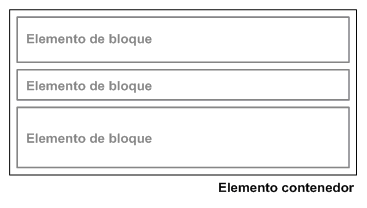
\includegraphics[width=0.8\textwidth]{figs/f0502.png}
\end{figure}
\end{center}

\end{frame}


%%---------------------------------------------------------------

\begin{frame}
\frametitle{Posicionamiento normal (o est�tico) (y II)}

\begin{itemize}
  \item Los elementos en l�nea forman los ``contextos de formato en l�nea''. Las cajas se muestran una detr�s de otra de forma horizontal comenzando desde la posici�n m�s a la izquierda de su elemento contenedor.
  \item Si las cajas en l�nea ocupan m�s espacio del disponible en su propia l�nea, el resto de cajas se muestran en las l�neas inferiores. 
  \item Si las cajas en l�nea ocupan un espacio menor que su propia l�nea, se puede controlar la distribuci�n de las cajas mediante la propiedad text-align para centrarlas, alinearlas a la derecha o justificarlas.
\end{itemize}


\begin{center}
\begin{figure}[p]
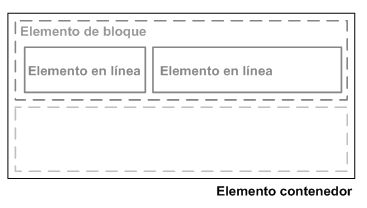
\includegraphics[width=0.8\textwidth]{figs/f0503.png}
\end{figure}
\end{center}

\end{frame}


%%---------------------------------------------------------------

\begin{frame}
\frametitle{Posicionamiento relativo}

\begin{itemize}
  \item Desplaza una caja respecto de su posici�n original establecida mediante el posicionamiento normal. El desplazamiento de la caja se controla con las propiedades top, right, bottom y left.
  \item la propiedad top se emplea para mover las cajas de forma descendente, la propiedad bottom mueve las cajas de forma ascendente, la propiedad left se utiliza para desplazar las cajas hacia la derecha y la propiedad right mueve las cajas hacia la izquierda. 
\end{itemize}

\begin{center}
\begin{figure}[p]
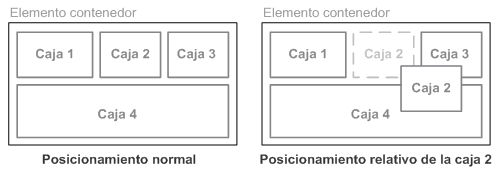
\includegraphics[width=0.8\textwidth]{figs/f0504.png}
\end{figure}
\end{center}

\end{frame}


%%---------------------------------------------------------------

\begin{frame}
\frametitle{Posicionamiento absoluto}

\begin{itemize}
  \item Se emplea para establecer de forma exacta la posici�n en la que se muestra la caja de un elemento. 
  \item Cuando una caja se posiciona de forma absoluta, el resto de elementos de la p�gina se ven afectados y modifican su posici�n. 
\end{itemize}

\begin{center}
\begin{figure}[p]
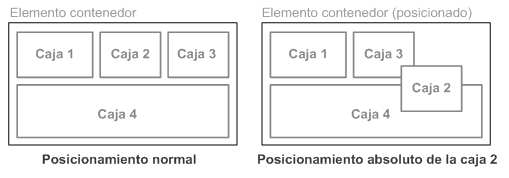
\includegraphics[width=0.8\textwidth]{figs/f0516.png}
\end{figure}
\end{center}

\end{frame}


%%---------------------------------------------------------------

\begin{frame}
\frametitle{Posicionamiento absoluto}

\begin{itemize}
  \item El primer elemento contenedor que est� posicionado de cualquier forma diferente a position: static se convierte en la referencia que determina la posici�n de la caja posicionada de forma absoluta.
  \item Si ning�n elemento contenedor est� posicionado, la referencia es la ventana del navegador, que no debe confundirse con el elemento $<body>$ de la p�gina.
  \item Una vez determinada la referencia del posicionamiento absoluto, la interpretaci�n de los valores de las propiedades top, right, bottom y left se realiza como sigue:
  \begin{itemize}
    \item Top: desplazamiento desde el borde superior del elemento contenedor que se utiliza como referencia.
    \item Right: �dem pero desde el borde derecho al borde derecho.
    \item Left:  �dem pero desde el borde izquierdo al borde izquierdo.
    \item Bottom: �dem pero desde el borde inferior al borde inferior.
  \end{itemize}
\end{itemize}

\end{frame}


%%---------------------------------------------------------------

\begin{frame}
\frametitle{Diferencias entre posicionamiento absoluto y relativo}

\begin{center}
\begin{figure}[p]
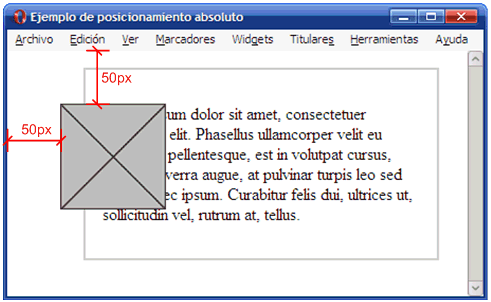
\includegraphics[width=0.6\textwidth]{figs/f0519.png}
\end{figure}
\end{center}

\begin{center}
\begin{figure}[p]
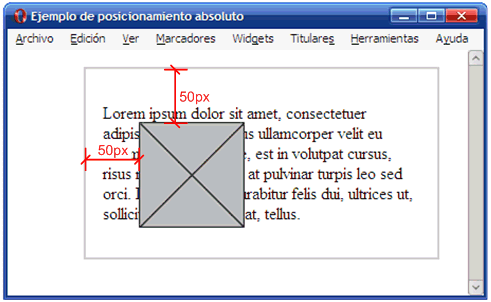
\includegraphics[width=0.6\textwidth]{figs/f0521.png}
\end{figure}
\end{center}

\end{frame}


%%---------------------------------------------------------------

\begin{frame}
\frametitle{Posicionamiento fijo}

\begin{itemize}
  \item Es un caso particular del posicionamiento absoluto, ya que s�lo se diferencian en el comportamiento de las cajas posicionadas.
  \item La principal caracter�stica de una caja posicionada de forma fija es que su posici�n es inamovible dentro de la ventana del navegador.
  \item El posicionamiento fijo hace que las cajas no modifiquen su posici�n ni aunque el usuario suba o baje la p�gina en la ventana de su navegador.
  \item Si la p�gina se visualiza en un medio paginado (por ejemplo en una impresora) las cajas posicionadas de forma fija se repiten en todas las p�ginas.
\end{itemize}

\end{frame}


%%---------------------------------------------------------------

\begin{frame}
\frametitle{Posicionamiento flotante}

\begin{itemize}
  \item Cuando una caja se posiciona con el modelo de posicionamiento flotante, autom�ticamente se convierte en una caja flotante, lo que significa que se desplaza hasta la zona m�s a la izquierda o m�s a la derecha de la posici�n en la que originalmente se encontraba.
\end{itemize}


\begin{center}
\begin{figure}[p]
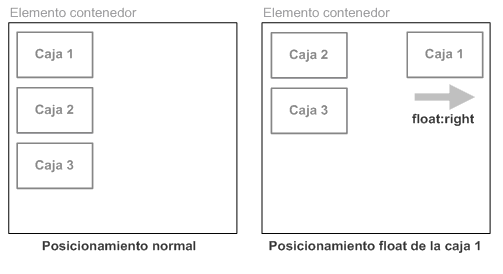
\includegraphics[width=0.8\textwidth]{figs/f0507.png}
\end{figure}
\end{center}

\end{frame}


%%---------------------------------------------------------------

\begin{frame}
\frametitle{Posicionamiento flotante (y II)}

\begin{itemize}
  \item Cuando se posiciona una caja de forma flotante:
  \begin{itemize}
    \item La caja deja de pertenecer al flujo normal de la p�gina, lo que significa que el resto de cajas ocupan el lugar dejado por la caja flotante.
    \item La caja flotante se posiciona lo m�s a la izquierda o lo m�s a la derecha posible de la posici�n en la que se encontraba originalmente.
  \end{itemize}
\end{itemize}


\begin{center}
\begin{figure}[p]
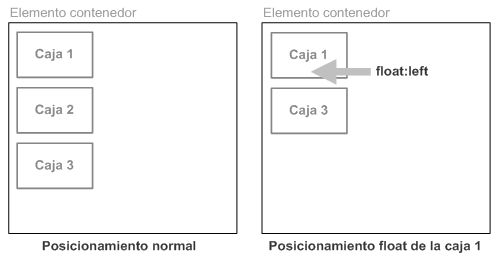
\includegraphics[width=0.8\textwidth]{figs/f0508.png}
\end{figure}
\end{center}

\end{frame}


%%---------------------------------------------------------------

\begin{frame}
\frametitle{Posicionamiento flotante (y III)}

\begin{itemize}
  \item Si existen otras cajas flotantes, al posicionar de forma flotante otra caja, se tiene en cuenta el sitio disponible.
  \item Si no existiera sitio en la l�nea actual, la caja flotante baja a la l�nea inferior hasta que encuentra el sitio necesario para mostrarse lo m�s a la izquierda o lo m�s a la derecha posible en esa nueva l�nea
\end{itemize}


\begin{center}
\begin{figure}[p]
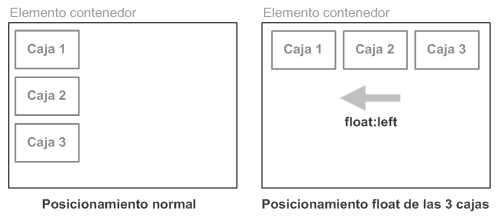
\includegraphics[width=0.8\textwidth]{figs/f0509.png}
\end{figure}
\end{center}

\end{frame}


%%---------------------------------------------------------------

\begin{frame}
\frametitle{Propiedad float}

\begin{center}
  \begin{table}
   \begin{tabular}{p{1.8cm}p{7.8cm}}
Propiedad & \bf{float} \\ \hline
Valores& left | right | none | inherit \\ \hline
Se aplica a& Todos los elementos \\ \hline
Valor inicial& none \\ \hline
Descripci�n& Establece el tipo de posicionamiento flotante del elemento \\ \hline
  \end{tabular}
   \caption{Definici�n de la propiedad float de CSS}
 \end{table}
\end{center}


\end{frame}


%%---------------------------------------------------------------

\begin{frame}
\frametitle{Posicionamiento flotante (y IV)}

\begin{itemize}
  \item Los elementos que se encuentran alrededor de una caja flotante adaptan sus contenidos para que fluyan alrededor del elemento posicionado
  \item Uno de los principales motivos para la creaci�n del posicionamiento float fue precisamente la posibilidad de colocar im�genes alrededor de las cuales fluye el texto.
\end{itemize}


\begin{center}
\begin{figure}[p]
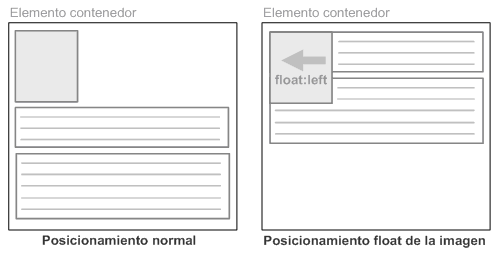
\includegraphics[width=0.8\textwidth]{figs/f0513.png}
\end{figure}
\end{center}

\end{frame}


%%---------------------------------------------------------------

\begin{frame}
\frametitle{Propiedad clear}

\begin{itemize}
  \item La propiedad clear indica el lado del elemento HTML que no debe ser adyacente a ninguna caja posicionada de forma flotante. Si se indica el valor left, el elemento se desplaza de forma descendente hasta que pueda colocarse en una l�nea en la que no haya ninguna caja flotante en el lado izquierdo.
  \item La especificaci�n oficial de CSS explica este comportamiento como ``un desplazamiento descendente hasta que el borde superior del elemento est� por debajo del borde inferior de cualquier elemento flotante hacia la izquierda''.
\end{itemize}

\end{frame}


%%---------------------------------------------------------------

\begin{frame}
\frametitle{Propiedad clear}

\begin{center}
  \begin{table}
   \begin{tabular}{p{1.8cm}p{7.8cm}}
Propiedad & \bf{clear} \\ \hline
Valores& none | left | right | both | inherit \\ \hline
Se aplica a& Todos los elementos de bloque \\ \hline
Valor inicial& none \\ \hline
Descripci�n& Indica el lado del elemento que no debe ser adyacente a ninguna caja flotante \\ \hline
  \end{tabular}
   \caption{Definici�n de la propiedad clear de CSS}
 \end{table}
\end{center}


\end{frame}



%%---------------------------------------------------------------

\begin{frame}
\frametitle{Propiedad display}

\begin{center}
  \begin{table}
   \begin{tabular}{p{1.8cm}p{7.8cm}}
Propiedad & \bf{display} \\ \hline
Valores& inline | block | none | list-item | run-in | inline-block | table | inline-table | table-row-group | table-header-group | table-footer-group | table-row | table-column-group | table-column | table-cell | table-caption | inherit \\ \hline
Se aplica a& Todos los elementos \\ \hline
Valor inicial& inline \\ \hline
Descripci�n& Permite controlar la forma de visualizar un elemento e incluso ocultarlo \\ \hline
  \end{tabular}
   \caption{Definici�n de la propiedad display de CSS}
 \end{table}
\end{center}


\end{frame}




%%---------------------------------------------------------------

\begin{frame}
\frametitle{Propiedad visibility}

\begin{center}
  \begin{table}
   \begin{tabular}{p{1.8cm}p{7.8cm}}
Propiedad & \bf{visibility} \\ \hline
Valores& visible | hidden | collapse | inherit \\ \hline
Se aplica a& Todos los elementos \\ \hline
Valor inicial& visible \\ \hline
Descripci�n& Permite hacer visibles e invisibles a los elementos \\ \hline
  \end{tabular}
   \caption{Definici�n de la propiedad visibility de CSS}
 \end{table}
\end{center}


\end{frame}


%%---------------------------------------------------------------

\begin{frame}
\frametitle{Propiedad overflow}

\begin{itemize}
  \item En algunas ocasiones el contenido de un elemento no cabe en el espacio reservado para ese elemento y se desborda.
  \item La situaci�n m�s habitual en la que el contenido sobresale de su espacio reservado es cuando se establece la anchura y/o altura de un elemento mediante la propiedad width y/o height. 
  \item Los valores de la propiedad overflow tienen el siguiente significado:
  \begin{itemize}
    \item visible: el contenido no se corta y se muestra sobresaliendo la zona reservada para visualizar el elemento. Este es el comportamiento por defecto.
    \item hidden: el contenido sobrante se oculta y s�lo se visualiza la parte del contenido que cabe dentro de la zona reservada para el elemento.
    \item scroll: solamente se visualiza el contenido que cabe dentro de la zona reservada para el elemento, pero tambi�n se muestran barras de scroll que permiten visualizar el resto del contenido.
    \item auto: el comportamiento depende del navegador, aunque normalmente es el mismo que la propiedad scroll.
  \end{itemize}
\end{itemize}

\end{frame}


%%---------------------------------------------------------------

\begin{frame}
\frametitle{Propiedad overflow (y II)}

\begin{center}
\begin{figure}[p]
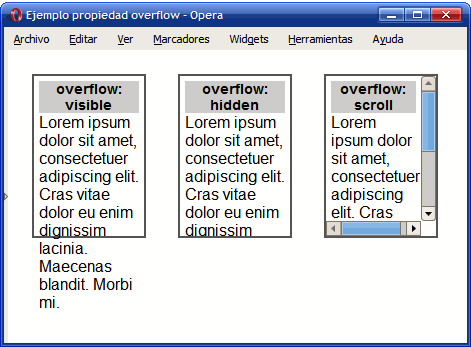
\includegraphics[width=0.8\textwidth]{figs/f0524.png}
\end{figure}
\end{center}

\end{frame}


%%---------------------------------------------------------------

\begin{frame}
\frametitle{Propiedad overflow (y III)}

\begin{center}
  \begin{table}
   \begin{tabular}{p{1.8cm}p{7.8cm}}
Propiedad & \bf{overflow} \\ \hline
Valores& visible | hidden | scroll | auto | inherit \\ \hline
Se aplica a& Elementos de bloque y celdas de tablas \\ \hline
Valor inicial& visible \\ \hline
Descripci�n& Permite controlar los contenidos sobrantes de un elemento \\ \hline
  \end{tabular}
   \caption{Definici�n de la propiedad overflow de CSS}
 \end{table}
\end{center}


\end{frame}



%%---------------------------------------------------------------

\begin{frame}
\frametitle{Propiedad z-index}

\begin{itemize}
  \item CSS permite controlar la posici�n tridimensional de las cajas posicionadas
  \item Es posible indicar las cajas que se muestran delante o detr�s de otras cajas cuando se producen solapamientos.
  \item Cuanto m�s alto sea el valor num�rico, m�s cerca del usuario se muestra la caja.
\end{itemize}

\end{frame}


%%---------------------------------------------------------------

\begin{frame}
\frametitle{Propiedad z-index (II)}


\begin{center}
\begin{figure}[p]
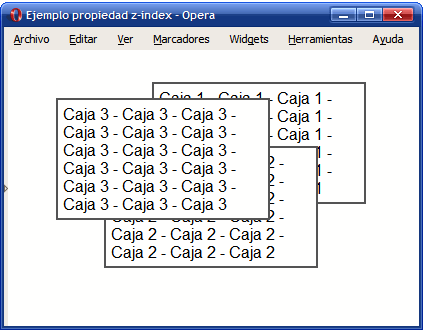
\includegraphics[width=0.66\textwidth]{figs/f0525.png}
\end{figure}
\end{center}

\end{frame}



%%---------------------------------------------------------------

\begin{frame}
\frametitle{Propiedad z-index (y III)}

\begin{center}
  \begin{table}
   \begin{tabular}{p{1.8cm}p{7.8cm}}
Propiedad & \bf{z-index} \\ \hline
Valores& auto | $<numero>$ | inherit \\ \hline
Se aplica a& Elementos que han sido posicionados expl�citamente \\ \hline
Valor inicial& auto \\ \hline
Descripci�n& Establece el nivel tridimensional en el que se muestra el elemento \\ \hline
  \end{tabular}
   \caption{Definici�n de la propiedad z-index de CSS}
 \end{table}
\end{center}


\end{frame}

%%---------------------------------------------------------------

\begin{frame}[fragile]
\frametitle{Selectores avanzados}

\begin{enumerate}
  \item Selector de hijos
\begin{verbatim}
p > span { color: blue; }
\end{verbatim}
  \item Selector adyacente
\begin{verbatim}
p + p { text-indent: 1.5em; }
\end{verbatim}
  \item Selector de atributos
\begin{verbatim}
a[class="externo"] { color: blue; }
a[class~="externo"] { color: blue; }
*[lang=en] { ... }
*[lang|="es"] { color : red }
\end{verbatim}
\end{enumerate}

\end{frame}



%%---------------------------------------------------------------

\begin{frame}
\frametitle{Colisi�n de estilos}

El m�todo seguido por CSS para resolver las colisiones de estilos se muestra a continuaci�n:

\begin{enumerate}
  \item Determinar todas las declaraciones que se aplican al elemento para el medio CSS seleccionado.
  \item Ordenar las declaraciones seg�n su origen (CSS de navegador, de usuario o de dise�ador) y su prioridad (palabra clave !important).
  \item Ordenar las declaraciones seg�n lo espec�fico que sea el selector. Cuanto m�s gen�rico es un selector, menos importancia tienen sus declaraciones.
  \item Si despu�s de aplicar las normas anteriores existen dos o m�s reglas con la misma prioridad, se aplica la que se indic� en �ltimo lugar.
\end{enumerate}

\end{frame}



%%---------------------------------------------------------------

\begin{frame}
\frametitle{Medios CSS}

\begin{itemize}
  \item Permiten definir diferentes estilos para diferentes medios o dispositivos: pantallas, impresoras, m�viles, proyectores, etc.
  \item Define algunas propiedades espec�ficamente para determinados medios: la paginaci�n y los saltos de p�gina para los medios impresos o el volumen y tipo de voz para los medios de audio.
  \item Ejemplos:
  \begin{itemize}
    \item screen: Pantallas de ordenador
    \item print: Impresoras y navegadores en el modo ``Vista Previa para Imprimir''
    \item handheld:	Dispositivos de mano: m�viles, PDA, etc.
  \end{itemize}
\end{itemize}

\end{frame}

%%---------------------------------------------------------------

\begin{frame}[fragile]
\frametitle{Formas de indicar el medio}

\begin{enumerate}
  \item Reglas de tipo @media
{\footnotesize
    \begin{verbatim}
@media print {
  body { font-size: 10pt }
}
@media screen {
  body { font-size: 13px }
}
    \end{verbatim}
}
  \item Reglas de tipo @import
{\footnotesize
    \begin{verbatim}
@import url("estilos_basicos.css") screen;
@import url("estilos_impresora.css") print;
    \end{verbatim}
}
  \item Medios definidos con la etiqueta
{\footnotesize
    \begin{verbatim}
<link rel="stylesheet" type="text/css" media="screen" href="basico.css" />
<link rel="stylesheet" type="text/css" media="print, handheld" href="especial.css" />
    \end{verbatim}
}
  \item Medios definidos mezclando varios m�todos
{\footnotesize
    \begin{verbatim}
<link rel="stylesheet" type="text/css"  media="screen" href="basico.css" />
@import url("estilos_seccion.css") screen;
@media print {
  /* Estilos espec�ficos para impresora */
}
    \end{verbatim}
}
\end{enumerate}

\end{frame}

%%---------------------------------------------------------------

\begin{frame}[fragile]
\frametitle{Comentarios}

\begin{itemize}
  \item El comienzo de un comentario se indica mediante los caracteres /* y el final del comentario se indica mediante */
    \begin{verbatim}
/* Este es un comentario en CSS */
    \end{verbatim}
  \item Pueden ocupar tantas l�neas como sea necesario, pero no se puede incluir un comentario dentro de otro comentario
    \begin{verbatim}
/* Este es un
   comentario CSS de varias
   lineas */
    \end{verbatim}
\end{itemize}

\end{frame}


%%---------------------------------------------------------------
\subsubsection*{Texto}

\begin{frame}
\frametitle{Tipograf�a}

\begin{itemize}
  \item CSS define numerosas propiedades para modificar la apariencia del texto
  \item color se utiliza para establecer el color de la letra
  \item Como el valor de la propiedad color se hereda, normalmente se establece la propiedad color en el elemento body para establecer el color de letra de todos los elementos de la p�gina
 \item font-family se utiliza para indicar el tipo de letra con el que se muestra el texto
  \item Suele definirse como una lista de tipos de letra alternativos separados por comas. El �ltimo valor de la lista es el nombre de la familia tipogr�fica gen�rica que m�s se parece al tipo de letra que se quiere utilizar.
\end{itemize}

\end{frame}


%%---------------------------------------------------------------

\begin{frame}
\frametitle{Propiedad color}

\begin{center}
  \begin{table}
   \begin{tabular}{p{1.8cm}p{7.8cm}}
Propiedad & \bf{color} \\ \hline
Valores& $<color>$ | inherit \\ \hline
Se aplica a& Todos los elementos \\ \hline
Valor inicial& Depende del navegador \\ \hline
Descripci�n& Establece el color de letra utilizado para el texto \\ \hline
  \end{tabular}
   \caption{Definici�n de la propiedad color de CSS}
 \end{table}
\end{center}


\end{frame}


%%---------------------------------------------------------------

\begin{frame}
\frametitle{Propiedad font-family}

\begin{center}
  \begin{table}
   \begin{tabular}{p{1.8cm}p{7.8cm}}
Propiedad & \bf{font-family} \\ \hline
Valores& (( $<nombre\_familia>$ | $<familia\_generica>$ ) (,$nombre\_familia>$ | $<familia\_generica$)* ) | inherit \\ \hline
Se aplica a& Todos los elementos \\ \hline
Valor inicial& Depende del navegador \\ \hline
Descripci�n& Establece el tipo de letra utilizado para el texto \\ \hline
  \end{tabular}
   \caption{Definici�n de la propiedad font-family de CSS}
 \end{table}
\end{center}


\end{frame}


%%---------------------------------------------------------------

\begin{frame}
\frametitle{Propiedad font-size (I)}

\begin{itemize}
  \item Adem�s de medida relativas, absolutas y de porcentajes, CSS permite utilizar una serie de palabras clave para indicar el tama�o de letra del texto:
  \begin{itemize}
    \item tama�o\_absoluto: indica el tama�o de letra de forma absoluta mediante alguna de las siguientes palabras clave: xx-small, x-small, small, medium, large, x-large, xx-large.
    \item tama�o\_relativo: indica de forma relativa el tama�o de letra del texto mediante dos palabras clave (larger, smaller) que toman como referencia el tama�o de letra del elemento padre.
  \end{itemize}
\end{itemize}


\begin{center}
\begin{figure}[p]
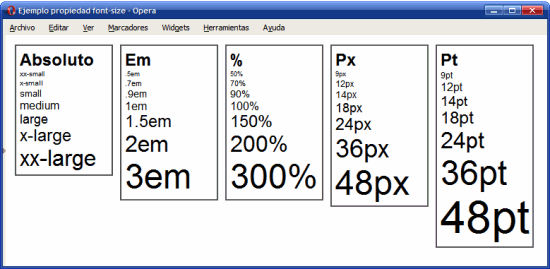
\includegraphics[width=0.6\textwidth]{figs/f0601.png}
\end{figure}
\end{center}

\end{frame}


%%---------------------------------------------------------------

\begin{frame}
\frametitle{Propiedad font-size (y II)}

\begin{center}
  \begin{table}
   \begin{tabular}{p{1.8cm}p{7.8cm}}
Propiedad & \bf{font-size} \\ \hline
Valores & $<tamano\_absoluto>$ | $<tamano\_relativo>$ | $<medida>$ | $<porcentaje>$ | inherit \\ \hline
Se aplica a & Todos los elementos \\ \hline
Valor inicial & medium \\ \hline
Descripci�n & Establece el tama�o de letra utilizado para el texto \\ \hline
  \end{tabular}
   \caption{Definici�n de la propiedad font-size de CSS}
 \end{table}
\end{center}

\end{frame}


%%---------------------------------------------------------------

\begin{frame}
\frametitle{Propiedad font-weight}

\begin{center}
  \begin{table}
   \begin{tabular}{p{1.8cm}p{7.8cm}}
Propiedad & \bf{font-weight} \\ \hline
Valores& normal | bold | bolder | lighter | 100 | 200 | 300 | 400 | 500 | 600 | 700 | 800 | 900 | inherit \\ \hline
Se aplica a& Todos los elementos \\ \hline
Valor inicial& normal \\ \hline
Descripci�n& Establece la anchura de la letra utilizada para el texto \\ \hline
  \end{tabular}
   \caption{Definici�n de la propiedad font-weight de CSS}
 \end{table}
\end{center}


\end{frame}


%%---------------------------------------------------------------

\begin{frame}
\frametitle{Propiedad font-style}

\begin{center}
  \begin{table}
   \begin{tabular}{p{1.8cm}p{7.8cm}}
Propiedad & \bf{font-style} \\ \hline
Valores& normal | italic | oblique | inherit \\ \hline
Se aplica a& Todos los elementos \\ \hline
Valor inicial& normal \\ \hline
Descripci�n& Establece el estilo de la letra utilizada para el texto \\ \hline
  \end{tabular}
   \caption{Definici�n de la propiedad font-style de CSS}
 \end{table}
\end{center}

\end{frame}


%%---------------------------------------------------------------

\begin{frame}
\frametitle{Propiedad font-variant}

\begin{center}
  \begin{table}
   \begin{tabular}{p{1.8cm}p{7.8cm}}
Propiedad & \bf{font-variant} \\ \hline
Valores& normal | small-caps | inherit \\ \hline
Se aplica a& Todos los elementos \\ \hline
Valor inicial& normal \\ \hline
Descripci�n& Establece el estilo alternativo de la letra utilizada para el texto \\ \hline
  \end{tabular}
   \caption{Definici�n de la propiedad font-variant de CSS}
 \end{table}
\end{center}


\end{frame}


%%---------------------------------------------------------------

\begin{frame}
\frametitle{Propiedad \emph{short-hand} font}

\begin{center}
  \begin{table}
   \begin{tabular}{p{1.8cm}p{7.8cm}}
Propiedad & \bf{font} \\ \hline
Valores& ( ( $<font-style>$ || $<font-variant>$ || $<font-weight>$ )? $<font-size>$ ( / $<line-height>$ )? $<font-family>$ ) | caption | icon | menu | message-box | small-caption | status-bar | inherit \\ \hline
Se aplica a& Todos los elementos \\ \hline
Valor inicial& - \\ \hline
Descripci�n& Permite indicar de forma directa todas las propiedades de la tipograf�a de un texto \\ \hline
  \end{tabular}
   \caption{Definici�n de la propiedad font de CSS}
 \end{table}
\end{center}


\end{frame}


%%---------------------------------------------------------------

\begin{frame}[fragile]
\frametitle{Propiedad \emph{short-hand} font (y II)}

\begin{itemize}
  \item El orden en el que se deben indicar las propiedades del texto es el siguiente:
  \begin{itemize}
    \item En primer lugar y de forma opcional se indican el font-style, font-variant y font-weight en cualquier orden.
    \item A continuaci�n, se indica obligatoriamente el valor de font-size seguido opcionalmente por el valor de line-height.
    \item Por �ltimo, se indica obligatoriamente el tipo de letra a utilizar.
  \end{itemize}
\end{itemize}

\begin{footnotesize}
\begin{verbatim}
font: bold 1em "Trebuchet MS",Arial,Sans-Serif;
font: normal 0.9em "Lucida Grande", Verdana, Arial, Helvetica, sans-serif;
font: normal 1.2em/1em helvetica, arial, sans-serif;
\end{verbatim}
\end{footnotesize}

\end{frame}


%%---------------------------------------------------------------

\begin{frame}
\frametitle{Texto}

\begin{itemize}
  \item Adem�s de las propiedades relativas a la tipograf�a del texto, CSS define numerosas propiedades que determinan la apariencia del texto en su conjunto.
  \item Estas propiedades adicionales permiten controlar
  \begin{itemize}
    \item la alineaci�n del texto,
    \item el interlineado,
    \item la separaci�n entre palabras,
    \item etc.
  \end{itemize}
\end{itemize}

\end{frame}


%%---------------------------------------------------------------

\begin{frame}
\frametitle{Propiedad text-align}

\begin{center}
  \begin{table}
   \begin{tabular}{p{1.8cm}p{7.8cm}}
Propiedad & \bf{text-align} \\ \hline
Valores& left | right | center | justify | inherit \\ \hline
Se aplica a& Elementos de bloque y celdas de tabla \\ \hline
Valor inicial& left \\ \hline
Descripci�n& Establece la alineaci�n del contenido del elemento \\ \hline
  \end{tabular}
   \caption{Definici�n de la propiedad text-align de CSS}
 \end{table}
\end{center}


\end{frame}


%%---------------------------------------------------------------

\begin{frame}
\frametitle{Propiedad line-height}

\begin{center}
  \begin{table}
   \begin{tabular}{p{1.8cm}p{7.8cm}}
Propiedad & \bf{line-height} \\ \hline
Valores& normal | $<numero>$ | $<medida>$ | $<porcentaje>$ | inherit \\ \hline
Se aplica a& Todos los elementos \\ \hline
Valor inicial& normal \\ \hline
Descripci�n& Permite establecer la altura de l�nea de los elementos \\ \hline
  \end{tabular}
   \caption{Definici�n de la propiedad line-height de CSS}
 \end{table}
\end{center}


\end{frame}


%%---------------------------------------------------------------

\begin{frame}
\frametitle{Propiedad text-decoration}

\begin{center}
  \begin{table}
   \begin{tabular}{p{1.8cm}p{7.8cm}}
Propiedad & \bf{text-decoration} \\ \hline
Valores& none | ( underline || overline || line-through || blink ) | inherit \\ \hline
Se aplica a& Todos los elementos \\ \hline
Valor inicial& none \\ \hline
Descripci�n& Establece la decoraci�n del texto (subrayado, tachado, parpadeante, etc.) \\ \hline
  \end{tabular}
   \caption{Definici�n de la propiedad text-decoration de CSS}
 \end{table}
\end{center}


\end{frame}


%%---------------------------------------------------------------

\begin{frame}
\frametitle{Propiedad text-transform}

\begin{center}
  \begin{table}
   \begin{tabular}{p{1.8cm}p{7.8cm}}
Propiedad & \bf{text-transform} \\ \hline
Valores& capitalize | uppercase | lowercase | none | inherit \\ \hline
Se aplica a& Todos los elementos \\ \hline
Valor inicial& none \\ \hline
Descripci�n& Transforma el texto original (lo transforma a may�sculas, a min�sculas, etc.) \\ \hline
  \end{tabular}
   \caption{Definici�n de la propiedad text-transform de CSS}
 \end{table}
\end{center}


\end{frame}


%%---------------------------------------------------------------

\begin{frame}
\frametitle{Propiedad vertical-align}

\begin{center}
  \begin{table}
   \begin{tabular}{p{1.8cm}p{7.8cm}}
Propiedad & \bf{vertical-align} \\ \hline
Valores& baseline | sub | super | top | text-top | middle | bottom | text-bottom | $<porcentaje>$ | $<medida>$ | inherit \\ \hline
Se aplica a& Elementos en l�nea y celdas de tabla \\ \hline
Valor inicial& baseline \\ \hline
Descripci�n& Determina la alineaci�n vertical de los contenidos de un elemento \\ \hline
  \end{tabular}
   \caption{Definici�n de la propiedad vertical-align de CSS}
 \end{table}
\end{center}


\end{frame}


%%---------------------------------------------------------------

\begin{frame}
\frametitle{Propiedad text-indent}

\begin{center}
  \begin{table}
   \begin{tabular}{p{1.8cm}p{7.8cm}}
Propiedad & \bf{text-indent} \\ \hline
Valores& $<medida>$ | $<porcentaje>$ | inherit \\ \hline
Se aplica a& Los elementos de bloque y las celdas de tabla \\ \hline
Valor inicial& 0 \\ \hline
Descripci�n& Tabula desde la izquierda la primera l�nea del texto original \\ \hline
  \end{tabular}
   \caption{Definici�n de la propiedad text-indent de CSS}
 \end{table}
\end{center}


\end{frame}


%%---------------------------------------------------------------

\begin{frame}
\frametitle{Propiedad letter-spacing}

\begin{center}
  \begin{table}
   \begin{tabular}{p{1.8cm}p{7.8cm}}
Propiedad & \bf{letter-spacing} \\ \hline
Valores& normal | $<medida>$ | inherit \\ \hline
Se aplica a& Todos los elementos \\ \hline
Valor inicial& normal \\ \hline
Descripci�n& Permite establecer el espacio entre las letras que forman las palabras del texto \\ \hline
  \end{tabular}
   \caption{Definici�n de la propiedad letter-spacing de CSS}
 \end{table}
\end{center}


\end{frame}


%%---------------------------------------------------------------

\begin{frame}
\frametitle{Propiedad word-spacing}

\begin{center}
  \begin{table}
   \begin{tabular}{p{1.8cm}p{7.8cm}}
Propiedad & \bf{word-spacing} \\ \hline
Valores& normal | $<medida>$ | inherit \\ \hline
Se aplica a& Todos los elementos \\ \hline
Valor inicial& normal \\ \hline
Descripci�n& Permite establecer el espacio entre las palabras que forman el texto \\ \hline
  \end{tabular}
   \caption{Definici�n de la propiedad word-spacing de CSS}
 \end{table}
\end{center}


\end{frame}


%%---------------------------------------------------------------

\begin{frame}
\frametitle{Propiedad white-space}

\begin{center}
  \begin{table}
   \begin{tabular}{p{1.8cm}p{7.8cm}}
Propiedad & \bf{white-space} \\ \hline
Valores& normal | pre | nowrap | pre-wrap | pre-line | inherit \\ \hline
Se aplica a& Todos los elementos \\ \hline
Valor inicial& normal \\ \hline
Descripci�n& Establece el tratamiento de los espacios en blanco del texto \\ \hline
  \end{tabular}
   \caption{Definici�n de la propiedad white-space de CSS}
 \end{table}
\end{center}


\end{frame}


%%---------------------------------------------------------------

\begin{frame}
\frametitle{Propiedad white-space (y II)}

El significado de cada uno de los valores es el siguiente:
\begin{itemize}
  \item normal: comportamiento por defecto de HTML.
  \item pre: se respetan los espacios en blanco y las nuevas l�neas (exactamente igual que la etiqueta $<pre>$). Si la l�nea es muy larga, se sale del espacio asignado para ese contenido.
  \item nowrap: elimina los espacios en blanco y las nuevas l�neas. Si la l�nea es muy larga, se sale del espacio asignado para ese contenido.
  \item pre-wrap: se respetan los espacios en blanco y las nuevas l�neas, pero ajustando cada l�nea al espacio asignado para ese contenido.
  \item pre-line: elimina los espacios en blanco y respeta las nuevas l�neas, pero ajustando cada l�nea al espacio asignado para ese contenido.
\end{itemize}

\end{frame}



%%---------------------------------------------------------------

\subsubsection*{Listas}

\begin{frame}
\frametitle{Propiedad list-style-type}

\begin{center}
  \begin{table}
   \begin{tabular}{p{1.8cm}p{7.8cm}}
Propiedad & \bf{list-style-type} \\ \hline
Valores& disc | circle | square | decimal | decimal-leading-zero | lower-roman | upper-roman | lower-greek | lower-latin | upper-latin | armenian | georgian | lower-alpha | upper-alpha | none | inherit \\ \hline
Se aplica a& Elementos de una lista \\ \hline
Valor inicial& disc \\ \hline
Descripci�n& Permite establecer el tipo de vi�eta mostrada para una lista \\ \hline
  \end{tabular}
   \caption{Definici�n de la propiedad list-style-type de CSS}
 \end{table}
\end{center}


\end{frame}


%%---------------------------------------------------------------

\begin{frame}
\frametitle{Propiedad list-style-position}

\begin{center}
  \begin{table}
   \begin{tabular}{p{1.8cm}p{7.8cm}}
Propiedad & \bf{list-style-position} \\ \hline
Valores& inside | outside | inherit \\ \hline
Se aplica a& Elementos de una lista \\ \hline
Valor inicial& outside \\ \hline
Descripci�n& Permite establecer la posici�n de la vi�eta de cada elemento de una lista \\ \hline
  \end{tabular}
   \caption{Definici�n de la propiedad list-style-type de CSS}
 \end{table}
\end{center}


\end{frame}


%%---------------------------------------------------------------

\begin{frame}
\frametitle{Propiedad list-style-image}

\begin{center}
  \begin{table}
   \begin{tabular}{p{1.8cm}p{7.8cm}}
Propiedad & \bf{list-style-image} \\ \hline
Valores& $<url>$ | none | inherit \\ \hline
Se aplica a& Elementos de una lista \\ \hline
Valor inicial& none \\ \hline
Descripci�n& Permite reemplazar las vi�etas autom�ticas por una imagen personalizada \\ \hline
  \end{tabular}
   \caption{Definici�n de la propiedad list-style-image de CSS}
 \end{table}
\end{center}


\end{frame}


%%---------------------------------------------------------------

\begin{frame}
\frametitle{Propiedad \emph{shorthand} list-style}

\begin{center}
  \begin{table}
   \begin{tabular}{p{1.8cm}p{7.8cm}}
Propiedad & \bf{list-style} \\ \hline
Valores& ( $<list-style-type>$ || $<list-style-position>$ || $<list-style-image>$ ) | inherit \\ \hline
Se aplica a& Elementos de una lista \\ \hline
Valor inicial& - \\ \hline
Descripci�n& Propiedad que permite establecer de forma simult�nea todas las opciones de una lista \\ \hline
  \end{tabular}
   \caption{Definici�n de la propiedad list-style de CSS}
 \end{table}
\end{center}


\end{frame}




%%---------------------------------------------------------------

%\begin{frame}
%\frametitle{}

%\begin{itemize}
%  \item 
%\end{itemize}
%
%\end{frame}



%% $Id$
%

\section{Hojas de estilo CSS3}


%%---------------------------------------------------------------

\begin{frame}
\frametitle{�Qu� es CSS3?}

\begin{itemize}
  \item CSS3 ofrece una gran variedad de maneras nuevas para el dise�o de hojas de estilo
  \item Al ser tan amplio el desarrollo de CSS3, se ha dividido en m�dulos:
  \begin{itemize}
    \item El modelo de caja
    \item Listas
    \item Presentaci�n de hiperv�culos
    \item Voz
    \item Fondos y bordes
    \item Efectos de texto
    \item ...
  \end{itemize}
\end{itemize}

\end{frame}


%%---------------------------------------------------------------

\begin{frame}
\frametitle{CSS3 todav�a en desarrollo}

\begin{itemize}
  \item Hay m�dulos, la mayor�a, cuya especificaci�n no est� terminada
  \item Hay m�dulos terminados, pero los navegadores no los implementan
  \item Es muy importante conocer el estado de la implementaci�n en navegadores
  \item Hay navegadores que tienen reglas espec�ficas (temporales)
  \begin{itemize}
    \item Comprobar si est� implementado en \url{http://caniuse.com/}
  \end{itemize}
\end{itemize}

\end{frame}


%%---------------------------------------------------------------

\begin{frame}
\frametitle{�Qu� hay de nuevo en CSS3?}

\begin{itemize}
  \item Las buenas noticias son que CSS3
  \begin{itemize}
    \item es {\bf compatible hacia atr�s}
    \item Mantiene la {\bf misma filosof�a}
  \end{itemize}
  \item B�sicamente, CSS3 a�ade nuevos selectores y propiedades
  \item Algunas son funcionalidades nuevas (animaciones o gradientes),
y otras permiten dise�os m�s sencillos (p.ej. el uso de columnas)
\end{itemize}

\end{frame}


%%---------------------------------------------------------------

\begin{frame}[fragile]
\frametitle{Especificidades de navegadores}

P.ej. border-radius:

\begin{footnotesize}
\begin{verbatim}
.box {
  -moz-border-radius: 10px;
  -webkit-border-radius: 10px;
  border-radius: 10px;
}
\end{verbatim}
\end{footnotesize}

(�imaginaos lo que era antes conseguir bordes redondeados!)

\end{frame}


%%---------------------------------------------------------------

\begin{frame}[fragile]
\frametitle{M�dulo Selectores}

\begin{itemize}
  \item first-child: primer elemento de la etiqueta padre
  \item last-child: �ltimo elemento de la etiqueta padre
  \item nth-child: selecciona m�ltiples elementos seg�n su posici�n en el �rbol
\end{itemize}

\begin{footnotesize}
\begin{verbatim}
p:first-child {
    background-color: yellow;
}
box:last-child {
    padding: 12px;
} 
\end{verbatim}
\end{footnotesize}

\end{frame}


%%---------------------------------------------------------------

\begin{frame}[fragile]
\frametitle{M�dulo Colores}

\begin{itemize}
  \item opacity: indica la opacidad de un elemento
  \item rgba: indica la opacidad de un color con el ``alpha"
\end{itemize}

\begin{footnotesize}
\begin{verbatim}
  /* red with opacity */
 .box1 {background-color: rgba(255,0,0,0.3);}  
  /* green with opacity */
 .box2 {background-color: rgba(0,255,0,0.3);}  
  /* blue with opacity */
 .box3 {background-color: rgba(0,0,255,0.3);}  
\end{verbatim}
\end{footnotesize}

\end{frame}


%%---------------------------------------------------------------

\begin{frame}[fragile]
\frametitle{M�dulo Fuentes}

\begin{itemize}
  \item @font-face: permite utilizar fuentes no instaladas en el cliente
\end{itemize}

\begin{footnotesize}
\begin{verbatim}
@font-face {
  font-family: "Essays 1743";
  font-weight: bold;
  src: url("f/Essays1743-bold.woff") format("woff");
}
\end{verbatim}
\end{footnotesize}

\end{frame}


%%---------------------------------------------------------------

\begin{frame}
\frametitle{M�dulo Fondos}

\begin{itemize}
  \item Se puede a�adir m�s de una imagen como fondo
  \item border-radius: se pueden a�adir bordes redondeados
  \item box-shadow: incluye sombras en cajas
\end{itemize}

\end{frame}

% 1 - CSS2
% 2 - bordes redondeados
% 3 - text shadow abbr
% 4 - shadow
% 5 - transparente
% 6 - gradiente
% 7 - rgba en los bordes
% 8 - rotate (a�adiendo algo de margen)
% 9 - scale

%% $Id$
%

\section{HTML5}


%% LICENCIA DE REDISTRIBUCION DE LAS TRANSPAS
\frame{
~
\vspace{1cm}

\begin{flushright}
\copyright Mark Pilgrim \\
\copyright Gregorio Robles - Universidad Rey Juan Carlos \\
\vspace{1cm}

Algunos derechos reservados. Este art�culo se distribuye bajo
la licencia ``Reconocimiento 3.0 Espa�a'' de Creative Commons,
disponible en \\
{\small \url{http://creativecommons.org/licenses/by/3.0/es/deed.es}}
\vspace{1cm}

Este documento se basa en el libro ''Dive into HTML5'' \\
disponible en http://diveintohtml5.info/
\end{flushright}
}


%%---------------------------------------------------------------
%%---------------------------------------------------------------

\section{5 cosas sobre HTML5}

%%---------------------------------------------------------------

\begin{frame}
\frametitle{1. No es una �nica cosa grande}

\begin{itemize}
  \item HTML5 es una colecci�n de funcionalidades
  \item No hace falta buscar soporte completo, pero s� de las funcionalidades concretas
  \item HTML5 especifica tambi�n c�mo interactuar con JavaScript y DOM
\end{itemize}

\end{frame}

%%---------------------------------------------------------------

\begin{frame}
\frametitle{2. No hace falta tirar nada}

\begin{itemize}
  \item Se basa en HTML4
  \item Si una web funcionaba con HTML4, funcionar� con HTML5
  \item HTML5 extiende HTML4 
  \item Los navegadores antiguos tratar�n muchos elementos HTML5 como si no existieran
\end{itemize}

\end{frame}

%%---------------------------------------------------------------

\begin{frame}[fragile]
\frametitle{3. Es f�cil empezar}

\begin{itemize}
  \item Cambiar a HTML5 es sencillo
  \item En realidad, s�lo hay que cambiar el DOCTYPE:
\begin{verbatim}
<!DOCTYPE html>
\end{verbatim}
  \item Los elementos obsoletos de HTML4 todav�a se ver�n en HTML5
\end{itemize}

\end{frame}

%%---------------------------------------------------------------

\begin{frame}
\frametitle{4. Ya funciona (en l�neas generales)}

\begin{itemize}
  \item Los navegadores est�n haciendo un gran esfuerzo por incluir HTML5
  \item Mientras tanto, tendremos que estar atentos a la compatibilidad de los mismos
  \item Todav�a no est� totalmente estandarizado
  \item Hasta 2020 no se espera soporte completo
\end{itemize}

\end{frame}

%%---------------------------------------------------------------

\begin{frame}
\frametitle{5. Est� aqu� para quedarse}

\begin{itemize}
  \item Reemplaza otras tecnolog�as: Flash
  \item Sigue la tendencia de que todo va a la nube
  \item Sigue la tendencia de la ubicuidad
\end{itemize}

\end{frame}


%%---------------------------------------------------------------
%%---------------------------------------------------------------

\section{Algunos elementos HTML5}
%%---------------------------------------------------------------

\begin{frame}[fragile]
\frametitle{DOCTYPE}

\begin{itemize}
  \item Hasta ahora hab�a diferentes modos:
  \begin{itemize}
    \item Quirks Mode
    \item Standards Mode
    \item Almost Standards Mode
  \end{itemize}
  \item En HTML5, s�lo hace falta:
\begin{verbatim}
<!DOCTYPE html>
\end{verbatim}
\end{itemize}

\end{frame}

%%---------------------------------------------------------------

\begin{frame}[fragile]
\frametitle{El Elemento ra�z}

\begin{itemize}
  \item Antes:
\begin{verbatim}
<html xmlns="http://www.w3.org/1999/xhtml"
      lang="en"
      xml:lang="en">
\end{verbatim}
  \item Ahora:
\begin{verbatim}
<html lang="en">
\end{verbatim}
\end{itemize}

\end{frame}

%%---------------------------------------------------------------

\begin{frame}[fragile]
\frametitle{Codificaci�n de caracteres}

\begin{itemize}
  \item Si podemos, env�amos cabecera:
\begin{verbatim}
Content-Type: text/html; charset="utf-8"
\end{verbatim}
  \item Si no se puede, en HTML5s:
\begin{verbatim}
<meta charset="utf-8" />
\end{verbatim}

\end{itemize}

\end{frame}

%%---------------------------------------------------------------

\begin{frame}
\frametitle{Relaciones}

\begin{itemize}
  \item Hoja de estilo: rel=''stylesheet''
  \item Feed: rel=''alternate''
  \item Emoticono: rel=''shortcut icon''
  \item Serie de p�ginas:  rel=''start'', rel=''prev'', rel=''next''
  \item ...
\end{itemize}

\end{frame}

%%---------------------------------------------------------------

\begin{frame}
\frametitle{Elementos sem�nticos}

\begin{itemize}
  \item $<section>$
  \item $<nav>$
  \item $<article>$
  \item $<aside>$
  \item $<hgroup>$
  \item $<header>$
  \item $<footer>$
  \item $<time>$
  \item $<mark>$
\end{itemize}

\end{frame}

%%---------------------------------------------------------------

\begin{frame}[fragile]
\frametitle{�C�mo muestran los navegadores elementos desconocidos?}

\begin{itemize}
  \item Las etiquetas desconocidas se muestran como si fueran ''inline''
  \item Regla CSS para cambiar el comportamiento:
\begin{verbatim}
article,aside,details,figcaption,figure,
footer,header,hgroup,menu,nav,section {
    display:block;
}
\end{verbatim}

Las versiones antiguas de Internet Explorer son especialmente ''particulares''.

\end{itemize}

\end{frame}

%%---------------------------------------------------------------
%%---------------------------------------------------------------

\section{El canvas}
%%---------------------------------------------------------------

\begin{frame}[fragile]
\frametitle{La etiqueta canvas}

\begin{itemize}
  \item Elemento canvas
  \item Se ha de especificar un tama�o (width y height)
  \item Requiere un id para poder manipularla
  \item El canvas siempre empieza vac�o
\end{itemize}

\begin{verbatim}
<canvas id="a" width="300" height="225"></canvas>
\end{verbatim}

\end{frame}

%%---------------------------------------------------------------

\begin{frame}[fragile]
\frametitle{Pintemos algo}

\begin{verbatim}
function draw_b() {
  var b_canvas = document.getElementById("b");
  var b_context = b_canvas.getContext("2d");
  b_context.fillRect(50, 25, 150, 100);
}
\end{verbatim}

\end{frame}

%%---------------------------------------------------------------

\begin{frame}
\frametitle{Algunas cuestiones a la hora de pintar}

\begin{itemize}
  \item La propiedad \emph{fillStyle} puede ser cualquier color CSS (tambi�n un patr�n o un gradiente). Por defecto, es negro.
  \item fillRect(x, y, width, height) pinta un rect�ngulo relleno (con el color de \emph{fillStyle}).
  \item La propiedad \emph{strokeStyle} es como \emph{fillStyle} pero para l�neas.
  \item strokeRect(x, y, width, height) pinta un rect�ngulo con el estilo de \emph{strokeStyle}.
  \item clearRect(x, y, width, height) borra los p�xeles del rect�ngulo especificado.
\end{itemize}

\end{frame}

%%---------------------------------------------------------------

\begin{frame}
\frametitle{Sobre las coordenadas}

\begin{itemize}
  \item La coordenada (0,0) est� en la esquina superior izquierda del canvas
  \item El eje X crece hacia la derecha
  \item El eje Y crece hacia abajo (!!)
\end{itemize}

\end{frame}

%%---------------------------------------------------------------

\begin{frame}
\frametitle{Caminos}

\begin{itemize}
  \item beginPath(): empieza un nuevo camino
  \item moveTo(x, y): sit�a el l�piz en la coordenada especificada.
  \item lineTo(x, y): pinta una l�nea hasta la coordenada especificada.
  \item stroke(): dibuja (con el estilo de \emph{strokeStyle}).
  \item arc(x, y, radio, angulo\_comienzo, angulo\_final, direccion);
  \begin{itemize}
    \item angulo\_comienzo y angulo\_final pueden ser p.ej. Math.PI * 2
    \item direccion: false si en el sentido del reloj
  \end{itemize}
\end{itemize}

\end{frame}


%%---------------------------------------------------------------

\begin{frame}
\frametitle{Texto}

\begin{itemize}
  \item font: como \emph{font} de CSS.
  \item textAlign: como el \emph{text-align} de CSS.
  \item textBaseLine: top, hanging, middle, alphabetic, ideographic, o bottom.
  \item fillText(''texto'', x, y): introduce ''texto'' en la posici�n (x, y).
\end{itemize}

\end{frame}

%%---------------------------------------------------------------

\begin{frame}
\frametitle{Ejercicio: Pintemos un diagrama de coordenadas}

\begin{center}
\begin{figure}[p]
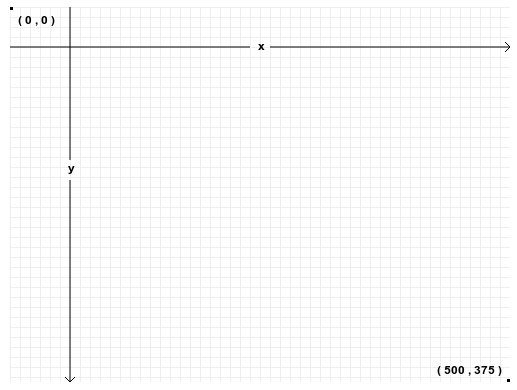
\includegraphics[width=0.8\textwidth]{figs/diagramacoordenadas.png}
\end{figure}
\end{center}

\end{frame}


%%---------------------------------------------------------------

\begin{frame}
\frametitle{Im�genes (I)}

\begin{itemize}
  \item drawImage(image, dx, dy): toma la imagen ''image'' y la pinta en el canvas. Las coordenadas dx y dy dan la esquina superior izquierda de la imagen.
  \item drawImage(image, dx, dy, dw, dh): toma la imagen ''image'' y la pinta en el canvas. Las coordenadas dx y dy dan la esquina superior izquierda de la imagen escal�ndola a una anchura dw y a una altura dh.
  \item drawImage(image, sx, sy, sw, sh, dx, dy, dw, dh): toma la imagen ''image'' y la introduce en el rect�ngulo (sx, sy, sw, sh), escal�ndola a las dimensiones (dw, dh), y la pinta en las coordenadas (dx, dy). V�ase la siguiente transparencia.
\end{itemize}

\end{frame}

%%---------------------------------------------------------------

\begin{frame}
\frametitle{Im�genes (y II)}

\begin{center}
\begin{figure}[p]
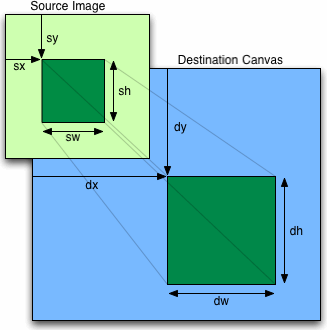
\includegraphics[width=0.6\textwidth]{figs/drawImage.png}
\end{figure}
\end{center}

\end{frame}

%%---------------------------------------------------------------
%%---------------------------------------------------------------

\section{Local Storage}

%%---------------------------------------------------------------

\begin{frame}
\frametitle{Buscando un espacio para guardar en local}

�Y por qu� no las cookies?

\begin{enumerate}
  \item Las cookies se incluyen en cada petici�n HTTP, ralentizando una aplicaci�n al enviarse una y otra vez
  \item Las cookies se incluyen en cada petici�n HTTP, enviando datos de manera no cifrada (a menos de que toda la aplicaci�n se sirva sobre SSL)
  \item Las cookies est�n limitadas a 4KB de datos - suficiente para ralentizar la conexi�n (v�ase punto 1), pero no lo suficiente para ser muy �tiles
\end{enumerate}

\end{frame}

%%---------------------------------------------------------------

\begin{frame}
\frametitle{HTML5 storage (Web storage)}

\begin{itemize}
  \item Es una manera de guardar parejas llave/valor de manera local, en el navegador cliente
  \item Estos datos persisten a�n cuando cerremos el navegador
  \item Estos datos no se transmiten al servidor, a menos de que se pidan de manera expl�cita
  \item Es un mecanismo implementado de manera nativa en navegadores web, evitando tener que utilizar plug-ins y otras extensiones/trucos.
\end{itemize}

\end{frame}

%%---------------------------------------------------------------

\begin{frame}[fragile]
\frametitle{Accediendo al almacenamiento local}

La intefaz:

\begin{verbatim}
interface Storage {
  getter any getItem(in DOMString key);
  setter creator void setItem(in DOMString key, in any data);
};
\end{verbatim}

Ejemplo de uso:
\begin{verbatim}
var foo = localStorage.getItem("bar");
// ...
localStorage.setItem("bar", foo);
\end{verbatim}

Tambi�n valdr�a:
\begin{verbatim}
var foo = localStorage["bar"];
// ...
localStorage["bar"] = foo;
\end{verbatim}

\end{frame}

%%---------------------------------------------------------------

\begin{frame}[fragile]
\frametitle{Borrando e iterando el almacenamiento local}

Interfaz de borrado:

\begin{verbatim}
interface Storage {
  deleter void removeItem(in DOMString key);
  void clear();
};
\end{verbatim}

Interfaz de iteraci�n:

\begin{verbatim}
interface Storage {
  readonly attribute unsigned long length;
  getter DOMString key(in unsigned long index);
};

\end{verbatim}


\end{frame}


%%---------------------------------------------------------------
%%---------------------------------------------------------------

\section{Navegaci�n Off-line}

%%---------------------------------------------------------------

\begin{frame}
\frametitle{Funcionamiento b�sico}

\begin{itemize}
  \item La p�gina web de una aplicaci�n off-line indicar� una lista (llamada {\bf manifest}) donde se indicar�n los archivos a descargarse
  \item Un navegador que implemente aplicaciones offline HTML5 leer� la lista del manifiesto y descargar� los archivos.
  \item El navegador se encargar� de tenerlos en cach� y actualizarlos si hay cambios
  \item Cuando se intente acceder a la aplicaci�n web sin conexi�n, entonces el navegador web autom�ticamente utilizar� las copias locales.
\end{itemize}

(hay un flag en el DOM que indica si estamos on-line u off-line)

\end{frame}

%%---------------------------------------------------------------

\begin{frame}[fragile]
\frametitle{El manifiesto}

�C�mo se indica el manififesto en una p�gina web?

\begin{verbatim}
<!DOCTYPE html>
<html manifest="/cache.manifest">
<body>
...
</body>
</html>
\end{verbatim}

El content-type del manifiesto ha de ser: text/cache-manifest .manifest

\end{frame}

%%---------------------------------------------------------------

\begin{frame}[fragile]
\frametitle{Un manifiesto sencillo}

Si tenemos un �nico archivo HTML, no hace falta indicarlo en el
manifiesto. Si son varios, entonces s� (adem�s de indicar el manifiesto
en cada una de las p�ginas).

\begin{verbatim}
CACHE MANIFEST
/clock.css
/clock.js
/clock-face.jpg
\end{verbatim}

Todos estos elementos est�n en la secci�n \emph{expl�cita}: 
se descargar�n y guardar�n en local.

\end{frame}

%%---------------------------------------------------------------

\begin{frame}[fragile]
\frametitle{La secci�n Network}

\begin{verbatim}
CACHE MANIFEST
NETWORK:
/tracking.cgi
CACHE:
/clock.css
/clock.js
/clock-face.jpg
\end{verbatim}

Elementos bajo la secci�n \emph{NETWORK} no se almacenan en local. La
secci�n \emph{expl�cita} pasa a indicarse como \emph{CACHE}.

\end{frame}

%%---------------------------------------------------------------

\begin{frame}[fragile]
\frametitle{La secci�n fallback}

Permite definir recursos que sustituyen a elementos en l�nea que por
la raz�n que sea no pueden ser almacenados en local (o no se almacenaron
con �xito): 

\begin{verbatim}
CACHE MANIFEST
FALLBACK:
/ /offline.html
NETWORK:
*
\end{verbatim}

\end{frame}

%%---------------------------------------------------------------
%%---------------------------------------------------------------

\section{Detecci�n de funcionalidad HTML5}

%%---------------------------------------------------------------

\begin{frame}
\frametitle{T�cnicas de detecci�n de caracter�sticas HTML5}

\begin{enumerate}
  \item Comprobar si existe una propiedad en un objeto global (como window o navigator). P.ej. geolocalizaci�n.
  \item  Crear un elemento y entonces comprobar si existe una propiedad espec�fica en ese elemento. P.ej. soporte para canvas.
  \item Crear un elemento, comprobor si existe un m�todo espec�fico en ese elemento y entonces llamar al m�todo y comprobar el valor de retorno. P.ej. comprobar formatos de v�deo soportados
  \item Crear un elemento, poner un valor a una propiedad, y comprobar si la propiedad ha retenido ese valor. P.ej. comprobar los tipos de $<input>$ soportados
  \item ... o utilizar la biblioteca JavaScript Modernizr
\end{enumerate}

\end{frame}

%%---------------------------------------------------------------

\begin{frame}[fragile]
\frametitle{Modernizr}

\begin{verbatim}
if (Modernizr.ELEMENT) {
  // let's go!
} else {
  // no native ELEMENT support available :(. 
  // Maybe try a fallback
}
\end{verbatim}

donde \emph{ELEMENT} puede ser: canvas, canvastext, video, video.webm, video.ogg, video.h264, localstorage, webworkers, applicationcache, geolocation, input.autofocus, history...

\end{frame}


%%---------------------------------------------------------------
%%---------------------------------------------------------------

\section{Geolocalizaci�n}


%%---------------------------------------------------------------

\begin{frame}[fragile]
\frametitle{Un ejemplo de geolocalizaci�n}

\begin{verbatim}
function get_location() {
  if (Modernizr.geolocation) {
    navigator.geolocation.getCurrentPosition(show_map);
  } else {
    // no native support; maybe try a fallback?
  }
}
\end{verbatim}

Geolocalizaci�n es opt-in para el usuario. Este c�digo ofrece un men� donde
puede compartir su geolocalizaci�n o no.

\end{frame}

%%---------------------------------------------------------------

\begin{frame}[fragile]
\frametitle{Sigamos con el ejemplo}

\begin{verbatim}
function show_map(position) {
  var latitude = position.coords.latitude;
  var longitude = position.coords.longitude;
  // let's show a map or do something interesting!
}
\end{verbatim}

La funci�n \emph{callback} se llamar� con un �nico par�metro: un objeto con dos
propiedades: \emph{coords} y \emph{timestamp}

\end{frame}

%%---------------------------------------------------------------

\begin{frame}
\frametitle{El objeto posici�n}

\begin{footnotesize}
\begin{tabular}{ l c l }
Propiedad & Tipo & Nota \\
\hline
coords.latitude	& double	& decimal degrees \\
coords.longitude & double	& decimal degrees \\
coords.altitude	& double or null	& meters above reference ellipsoid \\
coords.accuracy	& double	& meters \\
coords.altitudeAccuracy	& double or null	& meters \\
coords.heading	& double or null	& degrees clockwise from true north \\
coords.speed	& double or null	& meters/second \\
timestamp	& DOMTimeStamp	& like a Date() object \\
\end{tabular}
\end{footnotesize}

\end{frame}


%%---------------------------------------------------------------
%%---------------------------------------------------------------

\section{Web Workers}

%%---------------------------------------------------------------

\begin{frame}
\frametitle{�Qu� son?}

\begin{itemize}
  \item Scripts en JavaScript que se ejecutan en el \emph{background}
  \item Por tanto, no bloquean la p�gina (los navegadores suelen ser de un �nico hilo)
  \item Son parecidos a los \emph{threads} (�pero no comparten memoria!)
  \item Son relativamente pesados... s�lo deber�an utilizarse si van a realizar
tareas pesadas que hagan que el coste de iniciar uno (en memoria y en procesamiento)
valga la pena
  \item Los Web Workers no tienen acceso al DOM, se comunican con el programa principal mediante
env�o de mensajes.
\end{itemize}

\end{frame}


%%---------------------------------------------------------------

\begin{frame}[fragile]
\frametitle{�C�mo se lanzan?}

\begin{enumerate}

  \item Se instancia un objeto Worker, cuyo par�metro es una URL con el c�digo JavaScript
  La URL tiene las mismas limitaciones de seguridad que JavaScript.
  Se puede empotrar en c�digo JavaScript en la misma p�gina HTML, pero entonces hay que
crear un objeto URL.

  \begin{verbatim}
var worker = new Worker("worker.js");
  \end{verbatim}

  \item Se pasa un mensaje al Worker.
  Normalmente este mensaje estar� en formato JSON.

  \begin{verbatim}
worker.postMessage("Hello World!");
  \end{verbatim}
\end{enumerate}

\end{frame}


%%---------------------------------------------------------------

\begin{frame}[fragile]
\frametitle{�C�mo se lanzan? (y II)}

\begin{enumerate}
  \setcounter{enumi}{2}

  \item En caso de recibir un mensaje de respuesta, se captura el evento y se hace lo que queramos con los datos que
recibidos (nota: generalmente recibiremos un JSON):
  \begin{verbatim}
worker.onmessage = function(event) {
	console.log("Hemos recibido " + event.data);
	hacemosAlgo();
}
  \end{verbatim}

  \item Se da por cerrado el Worker:
  \begin{verbatim}
worker.terminate();
  \end{verbatim}
\end{enumerate}

\end{frame}


%%---------------------------------------------------------------
%%---------------------------------------------------------------

\section{WebSocket}

%%---------------------------------------------------------------

\begin{frame}
\frametitle{�Qu� son los WebSockets?}

\begin{itemize}
  \item Protocolo que permite tener comunicaci�n full-duplex sobre TCP (RFC 6455)
  \item Usa el puerto 80 (bueno para evitar firewalls)
  \item Es independiente de HTTP - el handshake es interpretado por los servidores como una petici�n \emph{Upgrade}
  \item Permite que el servidor env�e contenido al navegador sin que �ste la haya solicitado
  \item Antes de la estandarizaci�n por el W3C, la soluci�n pasaba por tecnolog�as como Comet
\end{itemize}

\end{frame}


%%---------------------------------------------------------------

\begin{frame}[fragile]
\frametitle{El \emph{handshake} con WebSockets}

{\bf Petici�n del cliente:}

\begin{verbatim}
GET /chat HTTP/1.1
Host: server.example.com
Upgrade: websocket
Connection: Upgrade
Sec-WebSocket-Key: x3JJHMbDL1EzLkh9GBhXDw==
Sec-WebSocket-Protocol: chat, superchat
Sec-WebSocket-Version: 13
Origin: http://example.com
\end{verbatim}

{\bf Respuesta del servidor:}

\begin{verbatim}
HTTP/1.1 101 Switching Protocols
Upgrade: websocket
Connection: Upgrade
Sec-WebSocket-Accept: HSmrc0sMlYUkAGmm5OPpG2HaGWk=
Sec-WebSocket-Protocol: chat
\end{verbatim}

\end{frame}


%%---------------------------------------------------------------

\begin{frame}[fragile]
\frametitle{Utilizando WebSockets}

\begin{enumerate}
  \item Instanciando un objeto WebSocket (n�tese que la URL empieza por 'ws'; tambi�n existe conexi�n segura mediante el uso de 'wss'):
\begin{verbatim}
var connection = new WebSocket('ws://gsyc.es/echo');
\end{verbatim}

  \item Enviamos datos al servidor (lo suyo ser�a enviar JSON, pero podemos enviar tambi�n otras cosas, como Blob o ArrayBuffer):
\begin{verbatim}
connection.onopen = function () {
  connection.send('Ping'); 
};
\end{verbatim}

\end{enumerate}

\end{frame}


%%---------------------------------------------------------------

\begin{frame}[fragile]
\frametitle{Utilizando WebSockets (y II)}

\begin{enumerate}
  \setcounter{enumi}{2}

  \item Podemos mirar si hay errores:
\begin{verbatim}
connection.onerror = function (error) {
  console.log('Error en el WebSocket: ' + error);
};
\end{verbatim}

  \item Recibimos del servidor (generalmente ser�n JSON, pero se pueden recibir otras cosas, como Blob o ArrayBuffer):
\begin{verbatim}
connection.onmessage = function (e) {
  console.log('Server: ' + e.data);
};
\end{verbatim}

\end{enumerate}

\end{frame}


%%---------------------------------------------------------------

\begin{frame}
\frametitle{Implementaciones en el servidor}

\begin{itemize}
  \item Node.js
  \begin{itemize}
    \item Socket.IO
    \item WebSocket-Node
    \item ws
  \end{itemize}
  \item Python
  \begin{itemize}
    \item pywebsocket
    \item Tornado
  \end{itemize}
  \item Java
  \begin{itemize}
    \item Jetty
  \end{itemize}
  \item Ruby
  \begin{itemize}
    \item EventMachine
  \end{itemize}
\end{itemize}
\end{frame}

%%---------------------------------------------------------------
%%---------------------------------------------------------------

\section{Firefox OS}

%%---------------------------------------------------------------

\begin{frame}
\frametitle{�Qu� es Firefox OS?}

\begin{itemize}
  \item Sistema operativo basado en Linux para \emph{smartphones} y tabletas
  \item Promovido por Mozilla (y otros \emph{partners} industriales
  \item Basado completamente en est�ndares abiertos: HTML5, CSS3 y JavaScript
  \item Incluye un modelo de privilegios y una API web abierta para comunicarse con el hardware del dispositivo
\end{itemize}

\end{frame}


%% $Id$
%

\section{La API de los servicios de Google}

%%---------------------------------------------------------------

\begin{frame}
\frametitle{La(s) API(s) de los servicios de Google}

\begin{itemize}
  \item Google ofrece una API para acceder a muchos servicios
  \item Algunas APIs son de pago
  \item Otras tienen limitaciones de uso gratuito
  \item Hay peticiones que requieren autenticaci�n y autorizaci�n
\end{itemize}

\end{frame}

%%---------------------------------------------------------------

\begin{frame}
\frametitle{El API Explorer (I)}

Google ofrece un servicio para explorar sus APIs, el API Explorer:

\begin{itemize}
  \item Permite conocer los m�todos de las APIs
  \item Permite probarlos mediante un formulario web
  \item A veces requieren autorizaci�n/autenticaci�n
  \item Incluyen un enlace a la documentaci�n completa
\end{itemize}

APIs Explorer: https://developers.google.com/apis-explorer/\#p/

\end{frame}


%%---------------------------------------------------------------

\begin{frame}
\frametitle{El API Explorer (II)}

\begin{center}
\begin{figure}[p]
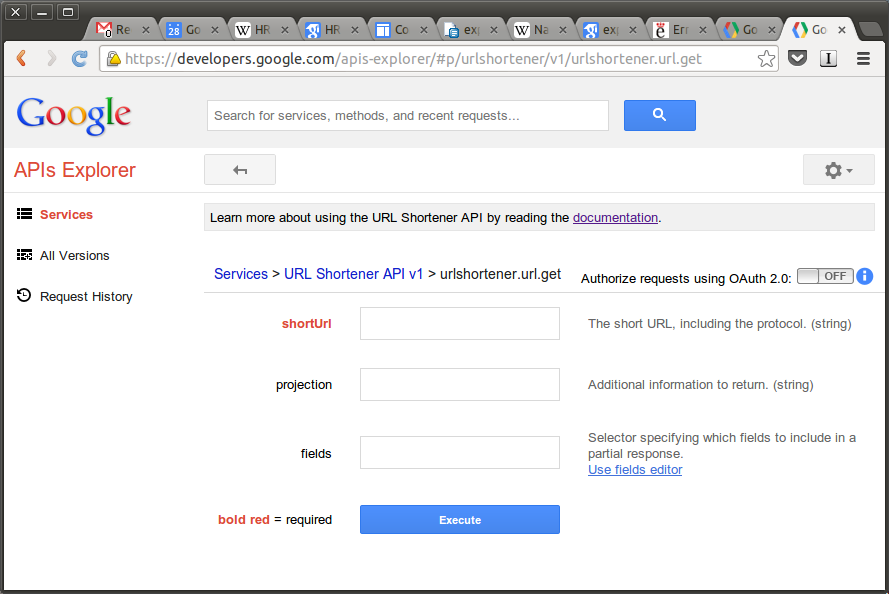
\includegraphics[width=0.8\textwidth]{figs/apiexplorer.png}
\end{figure}
\end{center}

\end{frame}

%%---------------------------------------------------------------

\begin{frame}
\frametitle{Ejemplo de uso del API Explorer}

Utilicemos el API Explorer para el servicio de acortadores de URLs de Google.

\begin{itemize}
  \item En el campo \emph{shortUrl}, introduce \emph{http://goo.gl/JCHYE}
  \item Pulsa el bot�n Execute
  \item Observa la petici�n: es una petici�n HTTP REST
  \item Observa la respuesta: es en formato JSON
\end{itemize}

\end{frame}

%%---------------------------------------------------------------

\begin{frame}
\frametitle{La Google API Console}

Es una interfaz web para gestionar el uso de la API de Google en tu proyecto.
Permite:

\begin{itemize}
  \item Activar APIs
  \item Obtener la llave (\emph{project key}) que se env�a al utilizar la API, gestionar autenticaci�n y autorizaci�n
  \item Obtener informaci�n de tr�fico (y ver las cuotas de uso)
  \item Gestionar cobros
  \item Gestionar miembros del equipo
\end{itemize}

\end{frame}


%%---------------------------------------------------------------

\begin{frame}
\frametitle{Ejercicio: Google API Console}

Crea un proyecto para utilizar la Google API Console.

\begin{itemize}
  \item Selecciona los servicios de Google+ API y URL Shortener API
  \item Obt�n tu \emph{project key}
  \item A�ade como \emph{referer} http://watson.gsyc.es/
  \item Incluye informaci�n de autorizaci�n v�a OAuth2.0, tambi�n para http://watson.gsyc.es/
  \item �chale un ojo a los men�s de \emph{Reports} y \emph{Quotas}
\end{itemize}

Nota: Para realizar este ejercicio (y los siguientes), necesitar�s tener
una cuenta en Google.

\end{frame}

\section{La API de Google+}

%%---------------------------------------------------------------

\begin{frame}[fragile]
\frametitle{La API de Google+}

\begin{itemize}
  \item Google+ ofrece una API REST para acceder a los contenidos de la red social
  \item Hay varios lenguajes soportados, entre ellos Javascript
  \item Los navegadores modernos lo soportan:
  \begin{itemize}
    \item Chrome 8+
    \item Firefox 3.5+
    \item MSIE 8+
    \item Safari 4+
  \end{itemize}
\end{itemize}


\end{frame}

%%---------------------------------------------------------------

\begin{frame}
\frametitle{Referencia de la API de Google+}

Hay cuatro tipo de recursos, que vienen representados con una estructura
de datos JSON:

\begin{itemize}
  \item People
  \item Activities
  \item Comments
  \item Moments
\end{itemize}

M�s informaci�n: https://developers.google.com/+/api/latest/

\end{frame}


%%---------------------------------------------------------------

\begin{frame}
\frametitle{Recursos}

Cada recurso cuenta con una serie de m�todos. Por ejempo, el recurso
People tiene:

\begin{itemize}
  \item get
  \item search
  \item listByActivity
  \item list
\end{itemize}

M�s informaci�n: https://developers.google.com/+/api/latest/people\#resource

\end{frame}


%%---------------------------------------------------------------

\begin{frame}
\frametitle{Estructura de un script Javascript}

\begin{enumerate}
  \item Se carga la biblioteca JavaScript
  \item Se indican los credenciales de acceso
  \item Se carga la API del servicio con el que queremos trabajar
  \item Se inicializa un objeto que encampsula la petici�n
  \item Se ejecuta el objeto petici�n
  \item Se procesa el resultado
\end{enumerate}

\end{frame}

%%---------------------------------------------------------------

\begin{frame}[fragile]
\frametitle{1. Cargando la biblioteca JavaScript}


\begin{footnotesize}
\begin{verbatim}
<script 
  src="https://apis.google.com/js/client.js?onload=OnLoadCallback">
</script>
\end{verbatim}
\end{footnotesize}

\begin{enumerate}
  \item Al producirse el evento, llama a la funci�n \emph{callback} que se indica
\end{enumerate}


\end{frame}

%%---------------------------------------------------------------

\begin{frame}
\frametitle{2. Indicando credenciales (I)}

Hay dos tipos de acceso:

\begin{enumerate}
  \item Simple:
  \begin{itemize}
    \item Llamadas que no acceden a datos privados
    \item Hace falta enviar la \emph{API key}
  \end{itemize}
  \item Autorizada:
  \begin{itemize}
    \item Llamadas que leen o escriben datos privados o de la propia aplicaci�n
    \item Hace falta un credencial OAuth 2.0
  \end{itemize}
\end{enumerate}

\end{frame}


%%---------------------------------------------------------------

\begin{frame}[fragile]
\frametitle{2. Indicando credenciales (I)}

Ejemplo de acceso simple:

\begin{footnotesize}
\begin{verbatim}
var apiKey = 'AIzaSyDy.......VbeXghdvuHDI8A'; // From API Console
gapi.client.setApiKey(apiKey);
\end{verbatim}
\end{footnotesize}

Ejemplo de acceso autorizado:

\begin{footnotesize}
\begin{verbatim}
// From the API Console
var clientId = '4764....7773'; 
// Services to be used
var scopes = 'https://www.googleapis.com/auth/plus.me'; 

gapi.auth.authorize({client_id: clientId, scope: scopes, immediate: true},
   callback_function);
\end{verbatim}
\end{footnotesize}

\texttt{callback\_function} es la funci�n que se ejecutar� una vez se haya obtenido
la autorizaci�n.

\end{frame}

%%---------------------------------------------------------------

\begin{frame}[fragile]
\frametitle{3. Cargar API del servicio}

\begin{verbatim}
gapi.client.load(API_NAME, API_VERSION, CALLBACK);
\end{verbatim}

donde:

\begin{itemize}
  \item API\_NAME es el nombre de la API
  \item API\_VERSION es la versi�n de la API
  \item CALLBACK es una funci�n opcional a ejecutar cuando se haya cargado
\end{itemize}

Para cargar la versi�n 1 de la API de Google+:

\begin{verbatim}
gapi.client.load('plus', 'v1', function() {
   console.log('loaded.'); 
});
\end{verbatim}

\end{frame}


%%---------------------------------------------------------------

\begin{frame}[fragile]
\frametitle{4. Objeto que encampsula petici�n}

\begin{verbatim}
var ApiRequest = gapi.client.METHOD_NAME(PARAMETERS_OBJECT);
\end{verbatim}

donde:

\begin{itemize}
  \item METHOD\_NAME es un m�todo de la API del servicio
  \item PARAMETERS\_OBJECT es un objeto con par�metros que depender�n 
del m�todo utilizado
\end{itemize}

Por ejemplo, la siguiente llamada busca actividades cuyo t�tulo sea Google+:

\begin{verbatim}
var request = gapi.client.plus.activities.search(
  {'query': 'Google+', 'orderBy': 'best'}
);
\end{verbatim}


\end{frame}


%%---------------------------------------------------------------

\begin{frame}[fragile]
\frametitle{5. Ejecuci�n del objeto petici�n}

\begin{verbatim}
ApiRequest.execute(callback);
\end{verbatim}

donde:

\begin{itemize}
  \item ApiRequest es un objeto que encapsula la petici�n (ver paso 4.)
  \item callback es la funci�n que tratar� la respuesta 
\end{itemize}

Por ejemplo:

\begin{verbatim}
request.execute(function(resp) { console.log(resp); });
\end{verbatim}

\end{frame}


%%---------------------------------------------------------------

\begin{frame}
\frametitle{6. Procesar el resultado}

\begin{itemize}
  \item La API devuelve dos objetos a la funci�n callback:
  \begin{enumerate}
    \item jsonResp: un objeto JSON
    \item rawResp: un string con la respuesta HTTP
  \end{enumerate}
\end{itemize}

Cuando la respuesta no pueda ofrecerse como JSON, el valor de jsonResp ser� \emph{false}; pero rawResp seguir� ofreciendo la respuesta HTTP completa como string.


\end{frame}





\end{document}
